\begin{filecontents*}{main.bib}
@inproceedings{karpukhin2020,
  title={Dense Passage Retrieval for Open-Domain Question Answering},
  author={Karpukhin, Vladimir and others},
  booktitle={Proceedings of the 2020 Conference on Empirical Methods in Natural Language Processing (EMNLP)},
  year={2020}
}

@article{izacard2022,
  title={Unsupervised Dense Information Retrieval with Contrastive Learning},
  author={Izacard, Gautier and others},
  journal={Transactions on Machine Learning Research (TMLR)},
  year={2022}
}

@inproceedings{zhan2021,
  title={Optimizing dense retrieval model training with hard negatives},
  author={Zhan, Jingtao and others},
  booktitle={Proceedings of the 44th International ACM SIGIR Conference on Research and Development in Information Retrieval},
  year={2021}
}

@inproceedings{thakur2021,
  title={BEIR: A Heterogeneous Benchmark for Zero-shot Evaluation of Information Retrieval Models},
  author={Thakur, Nandan and others},
  booktitle={Advances in Neural Information Processing Systems (NeurIPS)},
  year={2021}
}

@inproceedings{joachims2002,
  title={Optimizing Search Engines using Clickthrough Data},
  author={Joachims, Thorsten},
  booktitle={Proceedings of the eighth ACM SIGKDD international conference on Knowledge discovery and data mining},
  year={2002}
}

@article{afsar2022,
  title={Reinforcement Learning for Search, Recommendation, and Online Advertising: A Survey},
  author={Afsar, M. M. and Crump, T. and Far, B.},
  journal={ACM Computing Surveys},
  year={2022}
}

@inproceedings{christiano2017,
  title={Deep reinforcement learning from human preferences},
  author={Christiano, Paul F. and others},
  booktitle={Advances in Neural Information Processing Systems (NeurIPS)},
  year={2017}
}

@inproceedings{cunningham2024,
  title={Sparse Autoencoders Find Highly Interpretable Features in Language Models},
  author={Cunningham, Hoagy and others},
  booktitle={Proceedings of the International Conference on Learning Representations (ICLR)},
  year={2024}
}

@article{elhage2022,
  title={Toy Models of Superposition},
  author={Elhage, Nelson and others},
  journal={arXiv preprint arXiv:2209.10652},
  year={2022}
}

@article{bricken2023,
  title={Towards Monosemanticity: Decomposing Language Models With Dictionary Learning},
  author={Bricken, Trenton and others},
  journal={Transformer Circuits Thread},
  year={2023}
}

@article{schulman2017,
  title={Proximal Policy Optimization Algorithms},
  author={Schulman, John and Wolski, Filip and Dhariwal, Prafulla and Radford, Alec and Klimov, Oleg},
  journal={arXiv preprint arXiv:1707.06347},
  year={2017}
}

@article{hofmann2013,
  title={Balancing exploration and exploitation in listwise and pairwise learning to rank for information retrieval},
  author={Hofmann, Katja and Whiteson, Shimon and de Rijke, Maarten},
  journal={Information Retrieval},
  year={2013}
}

@inproceedings{wei2017,
  title={Reinforcement learning to rank with markov decision process},
  author={Wei, Zeng and others},
  booktitle={Proceedings of the 40th International ACM SIGIR Conference},
  year={2017}
}

@inproceedings{hu2018,
  title={Reinforcement learning to rank in e-commerce search engine: Formalization, analysis, and application},
  author={Hu, Yujing and others},
  booktitle={Proceedings of the 24th ACM SIGKDD International Conference},
  year={2018}
}

@inproceedings{nogueira2017,
  title={Task-Oriented Query Reformulation with Reinforcement Learning},
  author={Nogueira, Rodrigo and Cho, Kyunghyun},
  booktitle={Proceedings of the 2017 Conference on Empirical Methods in Natural Language Processing (EMNLP)},
  year={2017}
}

@inproceedings{buck2018,
  title={Ask the right questions: Active question reformulation with reinforcement learning},
  author={Buck, Christian and others},
  booktitle={International Conference on Learning Representations (ICLR)},
  year={2018}
}

@inproceedings{ouyang2021,
  title={Minimizing User Effort in Recommender Systems with Reinforcement Learning},
  author={Ouyang, Shiyao and others},
  booktitle={Proceedings of the 27th ACM SIGKDD Conference},
  year={2021}
}

@inproceedings{zou2019,
  title={Reinforcement Learning to Optimize Long-term User Engagement in Recommender Systems},
  author={Zou, Lixin and others},
  booktitle={Proceedings of the 25th ACM SIGKDD International Conference},
  year={2019}
}

@inproceedings{zheng2018,
  title={DRN: A Deep Reinforcement Learning Framework for News Recommendation},
  author={Zheng, Guanjie and others},
  booktitle={Proceedings of the 2018 World Wide Web Conference},
  year={2018}
}

@inproceedings{zhao2018,
  title={Deep Reinforcement Learning for Page-wise Recommendations},
  author={Zhao, Xiangyu and others},
  booktitle={Proceedings of the 12th ACM Conference on Recommender Systems},
  year={2018}
}

@inproceedings{chen2019,
  title={Top-K Off-Policy Correction for a REINFORCE Recommender System},
  author={Chen, Minmin and others},
  booktitle={Proceedings of the Twelfth ACM International Conference on Web Search and Data Mining},
  year={2019}
}

@inproceedings{yao2018,
  title={Reinforcement learning for dynamic reasoning in knowledge graphs},
  author={Yao, Liang and others},
  booktitle={Proceedings of the 56th Annual Meeting of the Association for Computational Linguistics},
  year={2018}
}

@inproceedings{ouyang2022,
  title={Training language models to follow instructions with human feedback},
  author={Ouyang, Long and others},
  booktitle={Advances in Neural Information Processing Systems (NeurIPS)},
  year={2022}
}

@inproceedings{stiennon2020,
  title={Learning to summarize from human feedback},
  author={Stiennon, Nisan and others},
  booktitle={Advances in Neural Information Processing Systems (NeurIPS)},
  year={2020}
}

@article{bai2022,
  title={Training a Helpful and Harmless Assistant with Reinforcement Learning from Human Feedback},
  author={Bai, Yuntao and others},
  journal={arXiv preprint arXiv:2204.05862},
  year={2022}
}

@article{ziegler2019,
  title={Fine-Tuning Language Models from Human Preferences},
  author={Ziegler, Daniel M. and others},
  journal={arXiv preprint arXiv:1909.08593},
  year={2019}
}

@article{olah2020,
  title={Zoom In: An Introduction to Circuits},
  author={Olah, Chris and others},
  journal={Distill},
  year={2020}
}

@article{goh2021,
  title={Multimodal Neurons in Artificial Neural Networks},
  author={Goh, Gabriel and others},
  journal={Distill},
  year={2021}
}

@inproceedings{yun2020,
  title={Transformer Feed-Forward Layers Are Key-Value Memories},
  author={Yun, Chulhee and others},
  booktitle={Proceedings of the 2020 Conference on Empirical Methods in Natural Language Processing (EMNLP)},
  year={2020}
}

@inproceedings{geva2022,
  title={Transformer Feed-Forward Layers Build Predictions by Promoting Concepts in the Vocabulary Space},
  author={Geva, Mor and others},
  booktitle={Proceedings of the 2022 Conference on Empirical Methods in Natural Language Processing},
  year={2022}
}

@inproceedings{meng2022,
  title={Locating and Editing Factual Associations in GPT},
  author={Meng, Kevin and others},
  booktitle={Advances in Neural Information Processing Systems (NeurIPS)},
  year={2022}
}

@article{templeton2024,
  title={Scaling Monosemanticity: Extracting Interpretable Features from Claude 3 Sonnet},
  author={Templeton, Adly and others},
  journal={Anthropic Research},
  year={2024}
}

@article{gao2024scaling,
  title={Scaling and evaluating sparse autoencoders},
  author={Gao, Leo and others},
  journal={arXiv preprint arXiv:2407.14956},
  year={2024}
}

@article{lee2023,
  title={Polysemanticity and Capacity in Neural Networks},
  author={Lee, Joonho and others},
  journal={arXiv preprint arXiv:2308.11896},
  year={2023}
}

@article{arora2018,
  title={Linear Algebraic Structure of Word Senses, with Applications to Polysemy},
  author={Arora, Sanjeev and others},
  journal={Transactions of the Association for Computational Linguistics},
  year={2018}
}

@inproceedings{conmy2023,
  title={Towards Automated Circuit Discovery for Mechanistic Interpretability},
  author={Conmy, Arthur and others},
  booktitle={Advances in Neural Information Processing Systems (NeurIPS)},
  year={2023}
}

@inproceedings{nanda2023,
  title={Progress measures for grokking via mechanistic interpretability},
  author={Nanda, Neel and others},
  booktitle={International Conference on Learning Representations (ICLR)},
  year={2023}
}

@inproceedings{wang2023,
  title={Interpretability in the Wild: a Circuit for Indirect Object Identification in GPT-2 small},
  author={Wang, Kevin and others},
  booktitle={International Conference on Learning Representations (ICLR)},
  year={2023}
}

@inproceedings{formal2021splade,
  title={SPLADE: Sparse Lexical and Expansion Model for First Stage Ranking},
  author={Formal, Thibault and Piwowarski, Benjamin and Clinchant, Stephane},
  booktitle={Proceedings of the 44th International ACM SIGIR Conference},
  year={2021}
}

@article{formal2021spladev2,
  title={SPLADE v2: Sparse Lexical and Expansion Model for Information Retrieval},
  author={Formal, Thibault and others},
  journal={arXiv preprint arXiv:2109.10086},
  year={2021}
}

@inproceedings{khattab2020,
  title={ColBERT: Efficient and Effective Passage Search via Contextualized Late Interaction over BERT},
  author={Khattab, Omar and Zaharia, Matei},
  booktitle={Proceedings of the 43rd International ACM SIGIR Conference},
  year={2020}
}

@inproceedings{santhanam2022,
  title={ColBERTv2: Effective and Efficient Retrieval via Lightweight Late Interaction},
  author={Santhanam, Keshav and others},
  booktitle={Proceedings of the 2022 Conference of the North American Chapter of the Association for Computational Linguistics},
  year={2022}
}

@inproceedings{robertson1994,
  title={Okapi at TREC-3},
  author={Robertson, Stephen E. and others},
  booktitle={Proceedings of the Third Text REtrieval Conference (TREC-3)},
  year={1994}
}

@article{nogueira2019,
  title={From doc2query to docTquery},
  author={Nogueira, Rodrigo and Lin, Jimmy},
  journal={arXiv preprint arXiv:1904.08375},
  year={2019}
}

@article{dai2019,
  title={Context-Aware Sentence/Passage Term Importance Estimation For First Stage Retrieval},
  author={Dai, Zhuyun and Callan, Jamie},
  journal={arXiv preprint arXiv:1910.10687},
  year={2019}
}

@article{lin2021,
  title={Pretrained Transformers for Text Ranking: BERT and Beyond},
  author={Lin, Jimmy and Nogueira, Rodrigo and Yates, Andrew},
  journal={Synthesis Lectures on Human Language Technologies},
  year={2021}
}

@article{luan2021,
  title={Sparse, Dense, and Attentional Representations for Text Retrieval},
  author={Luan, Yi and others},
  journal={Transactions of the Association for Computational Linguistics},
  year={2021}
}

@inproceedings{gao2021coil,
  title={CoIL: Revisit Exact Lexical Match in Information Retrieval with Contextualized Inverted List},
  author={Gao, Luyu and Callan, Jamie and Dai, Zhuyun},
  booktitle={Proceedings of the 2021 Conference of the North American Chapter of the Association for Computational Linguistics},
  year={2021}
}

@inproceedings{qu2021,
  title={RocketQA: An Optimized Training Approach to Dense Passage Retrieval for Open-Domain Question Answering},
  author={Qu, Yingqi and others},
  booktitle={Proceedings of the 2021 Conference of the North American Chapter of the Association for Computational Linguistics},
  year={2021}
}

@inproceedings{hofstatter2021,
  title={Efficiently Teaching an Effective Dense Retriever with Balanced Topic Aware Sampling},
  author={Hofst\"{a}tter, Sebastian and others},
  booktitle={Proceedings of the 44th International ACM SIGIR Conference},
  year={2021}
}

@inproceedings{xiong2021,
  title={Approximate Nearest Neighbor Negative Contrastive Learning for Dense Text Retrieval},
  author={Xiong, Lee and others},
  booktitle={International Conference on Learning Representations (ICLR)},
  year={2021}
}

@article{johnson2019,
  title={Billion-scale similarity search with GPUs},
  author={Johnson, Jeff and Douze, Matthijs and J{\'e}gou, Herv{\'e}},
  journal={IEEE Transactions on Big Data},
  year={2019}
}

@inproceedings{shrivastava2014,
  title={Asymmetric LSH (ALSH) for Sublinear Time Maximum Inner Product Search (MIPS)},
  author={Shrivastava, Anshumali and Li, Ping},
  booktitle={Advances in Neural Information Processing Systems (NeurIPS)},
  year={2014}
}

@inproceedings{beyer1999,
  title={When is 'nearest neighbor' meaningful?},
  author={Beyer, Kevin and others},
  booktitle={International Conference on Database Theory},
  year={1999}
}

@inproceedings{ethayarajh2019,
  title={How Contextual are Contextualized Word Representations?},
  author={Ethayarajh, Kawin},
  booktitle={Proceedings of the 2019 Conference on Empirical Methods in Natural Language Processing},
  year={2019}
}

@book{sutton2018,
  title={Reinforcement Learning: An Introduction},
  author={Sutton, Richard S. and Barto, Andrew G.},
  publisher={MIT Press},
  year={2018}
}

@article{olshausen1996,
  title={Emergence of simple-cell receptive field properties by learning a sparse code for natural images},
  author={Olshausen, Bruno A. and Field, David J.},
  journal={Nature},
  year={1996}
}

@inproceedings{glorot2011,
  title={Deep Sparse Rectifier Neural Networks},
  author={Glorot, Xavier and Bordes, Antoine and Bengio, Yoshua},
  booktitle={Proceedings of the Fourteenth International Conference on Artificial Intelligence and Statistics},
  year={2011}
}

@inproceedings{engstrom2020,
  title={Implementation Matters in Deep Policy Gradients: A Case Study on PPO and TRPO},
  author={Engstrom, I. and Ilyas, A. and Santurkar, S. and Tsipras, D. and Janoos, F. and Rudolph, L. and Madry, A.},
  booktitle={International Conference on Learning Representations (ICLR)},
  year={2020}
}

@inproceedings{konda1999,
  title={Actor-Critic Algorithms},
  author={Konda, Vijay R. and Tsitsiklis, John N.},
  booktitle={Advances in Neural Information Processing Systems (NeurIPS)},
  year={1999}
}

@inproceedings{ng1999,
  title={Policy invariance under reward transformations: Theory and application to reward shaping},
  author={Ng, Andrew Y. and Harada, Daishi and Russell, Stuart},
  booktitle={Proceedings of the Sixteenth International Conference on Machine Learning (ICML)},
  year={1999}
}

@inproceedings{lillicrap2016,
  title={Continuous control with deep reinforcement learning},
  author={Lillicrap, Timothy P. and others},
  booktitle={International Conference on Learning Representations (ICLR)},
  year={2016}
}

@inproceedings{schulman2016,
  title={High-Dimensional Continuous Control Using Generalized Advantage Estimation},
  author={Schulman, John and Moritz, Philipp and Levine, Sergey and Jordan, Michael and Abbeel, Pieter},
  booktitle={International Conference on Learning Representations (ICLR)},
  year={2016}
}

@article{williams1992,
  title={Simple statistical gradient-following algorithms for connectionist reinforcement learning},
  author={Williams, Ronald J.},
  journal={Machine Learning},
  year={1992}
}

@inproceedings{cohan2020,
  title={SPECTER: Document-level Representation Learning using Citation-informed Transformers},
  author={Cohan, Arman and others},
  booktitle={Proceedings of the 58th Annual Meeting of the Association for Computational Linguistics},
  year={2020}
}

@inproceedings{wachsmuth2018,
  title={Retrieval of the Best Counterargument without Prior Topic Knowledge},
  author={Wachsmuth, Henning and others},
  booktitle={Proceedings of the 56th Annual Meeting of the Association for Computational Linguistics},
  year={2018}
}

@inproceedings{boteva2016,
  title={A Full-Text Learning to Rank Dataset for Medical Information Retrieval},
  author={Boteva, Vera and others},
  booktitle={Advances in Information Retrieval},
  year={2016}
}

@inproceedings{maia2018,
  title={18th International Conference on Web Engineering (ICWE 2018) WWW'18 Companion: FinQA},
  author={Maia, Macedo and others},
  booktitle={Companion Proceedings of the The Web Conference 2018},
  year={2018}
}

@article{voorhees2021,
  title={TREC-COVID: Constructing a Pandemic Information Retrieval Test Collection},
  author={Voorhees, Ellen and others},
  journal={SIGIR Forum},
  year={2021}
}

@inproceedings{paszke2019,
  title={PyTorch: An Imperative Style, High-Performance Deep Learning Library},
  author={Paszke, Adam and others},
  booktitle={Advances in Neural Information Processing Systems (NeurIPS)},
  year={2019}
}

@article{jarvelin2002,
  title={Cumulated gain-based evaluation of IR techniques},
  author={J{\"a}rvelin, Kalervo and Kek{\"a}l{\"a}inen, Jaana},
  journal={ACM Transactions on Information Systems (TOIS)},
  year={2002}
}

@inproceedings{smucker2007,
  title={A comparison of statistical significance tests for information retrieval evaluation},
  author={Smucker, Mark D. and Allan, James and Carterette, Ben},
  booktitle={Proceedings of the 16th ACM conference on Conference on information and knowledge management},
  year={2007}
}

@article{baeza-yates2018,
  title={Bias on the Web},
  author={Baeza-Yates, Ricardo},
  journal={Communications of the ACM},
  year={2018}
}

@article{amodei2016,
  title={Concrete Problems in AI Safety},
  author={Amodei, Dario and others},
  journal={arXiv preprint arXiv:1606.06565},
  year={2016}
}

@inproceedings{skalse2022,
  title={Defining and Characterizing Reward Gaming},
  author={Skalse, Joar and others},
  booktitle={Advances in Neural Information Processing Systems (NeurIPS)},
  year={2022}
}

@inproceedings{broder2003,
  title={Efficient query evaluation using a two-level retrieval process},
  author={Broder, Andrei Z. and others},
  booktitle={Proceedings of the twelfth international conference on Information and knowledge management (CIKM)},
  year={2003}
}

@book{noble2018,
  title={Algorithms of Oppression: How Search Engines Reinforce Racism},
  author={Noble, Safiya Umoja},
  publisher={NYU Press},
  year={2018}
}

@inproceedings{craswell2008,
  title={An experimental comparison of click position-bias models},
  author={Craswell, Nick and others},
  booktitle={Proceedings of the 2008 international conference on web search and data mining},
  year={2008}
}

@inproceedings{macdonald2012,
  title={Learning to Predict Response Times for Online Query Scheduling},
  author={Macdonald, Craig and Tonellotto, Nicola and Ounis, Iadh},
  booktitle={Proceedings of the 35th International ACM SIGIR Conference},
  year={2012}
}

@inproceedings{joachims2017,
  title={Unbiased Learning-to-Rank with Biased Feedback},
  author={Joachims, Thorsten and others},
  booktitle={Proceedings of the Tenth ACM International Conference on Web Search and Data Mining (WSDM)},
  year={2017}
}
\end{filecontents*}

\begin{filecontents*}{rlj.sty}
% RLC rlj.sty Version 2026.1

% This style file was adapted from previous style files in the following reverse-chronological order:
% Adapted by Marlos C. Machado and Philip Thomas for RLJ/RLC 2026
% Adapted by Philip Thomas and Glen Berseth for RLJ/RLC 2024
% Adapted by Hugo Larochelle and Fabian Pedregosa for TMLR
% Adapted by ICLR, borrowing from JMLR.

% Last edited, October 2026 by Marlos C. Machado and Philip Thomas
%   - Implemented several changes for RLJ/RLC 2026

% First, include the packages we require
\RequirePackage{fancyhdr}   % For modifying the header
\RequirePackage{natbib}     % For formatting references
\RequirePackage{enumitem}   % For removing the indentetion in an enumerate block
\RequirePackage[T1]{fontenc}% T1 font encoding for hyphenation and accents
\RequirePackage{times}      % Set the font to times new roman
\RequirePackage{ragged2e}   % For justifying text on the title page
\RequirePackage{tcolorbox}  % For the colored box on the title page
\RequirePackage{hyperref}   % For hyperlinks (e.g., clicking references)
\RequirePackage{xcolor}     % For setting the color of links and boxes
\RequirePackage{lineno}     % For line numbers when in-submission
\RequirePackage{amsmath}    % <- after lineno
\RequirePackage{etoolbox}   % <- for \cspreto, \csappto, used in amsmath + lineno fix

% Slightly increase header height to avoid fancyhdr warning
\setlength{\headheight}{12.1001pt}

% modification to natbib citations
\setcitestyle{authoryear,round,citesep={;},aysep={,},yysep={;}}

% Make the links a blue color so that they are visually identifiable in digital forms.
\definecolor{dark-blue}{rgb}{0,0,0.7}
\hypersetup{
    colorlinks, linkcolor={dark-blue},
    citecolor={dark-blue}, urlcolor={dark-blue}
}

% Default max portion of a page for a float (e.g., figure) is 50%. Change to 95% to allow large figures.
\renewcommand{\topfraction}{0.95}

% Default minimum fraction of page that must be occupied by text is 20%. Change to 5% to help with float placement.
\renewcommand{\textfraction}{0.05}

% Create a conditional flag called '@accepted' and set its default value to 'false'
\newif\if@accepted\@acceptedfalse

% Define an option 'accepted' that sets the '@accepted' flag to 'true'
\DeclareOption{accepted}{%
    \@acceptedtrue
}

% Create another conditional flag called '@preprint' and set its default value to 'false'
\newif\if@preprint\@preprintfalse

% Define an option 'preprint' that sets both '@preprint' and '@accepted' flags to 'true'
% The 'preprint' option can be used to create a version ready for preprint uploads (e.g., to arXiv)
\DeclareOption{preprint}{
  \@preprinttrue
  \@acceptedtrue
}

% If an unrecognized option is passed to the 'rlj' package, issue a warning message.
\DeclareOption*{\PackageWarning{rlj}{Unknown ‘\CurrentOption’}}

% Process all the options that were passed to the 'rlj' package.
% This applies the declared options ('accepted', 'preprint', etc.) or triggers the fallback warning for unknown options.
\ProcessOptions\relax

% New commands to store emails and affiliations
\newcommand{\emails}[1]{\def\@emails{#1}}
\newcommand{\affiliations}[1]{\def\@affiliations{#1}}
\newcommand{\keywords}[1]{\gdef\@keywords{#1}}  % Define command to store keywords
\newcommand{\summary}[1]{\gdef\@summary{#1}}    % Define command to create summary
\newcommand{\coverPageAuthor}[1]{\def\@coverPageAuthor{#1}} % Define command to store cover page authors without superscripts

% Command to set and store the running title
\newcommand{\setrunningtitle}[1]{
    \def\therunningtitle{#1}  % Store the running title
    \markboth{#1}{}           % Set the running title in the header
}

% Specify the dimensions of each page
\setlength{\paperheight}{11in}
\setlength{\paperwidth}{8.5in}

\oddsidemargin 0.5in            % Set the left margin for odd-numbered pages to 0.5 inches.
\evensidemargin 0.5in           % Set the left margin for even-numbered pages to match the odd-numbered pages (for double-sided documents).
\marginparwidth 0in             % Disable margin notes by setting the margin width to 0.
\topmargin -0.5in               % Set the top margin to -0.5 inches to adjust the vertical position of the text area.
\textheight 9.0 true in         % Define the height of the text area, including footnotes and figures, to be 9 inches.
\textwidth 5.5 true in          % Define the width of the text area to be 5.5 inches.
\widowpenalty=10000             % Prevent single lines (widows) at the top of a page by assigning a high penalty.
\clubpenalty=10000              % Prevent single lines (orphans) at the bottom of a page by assigning a high penalty.
\flushbottom                    % Align the text at the bottom of each page to give pages a consistent length.
\sloppy                         % Allow LaTeX more flexibility in line-breaking to reduce overfull lines (long lines extending into the margins).
\def\addcontentsline#1#2#3{}    % Disable the creation of table of contents entries to save space, as they are not needed for this document.


\definecolor{customBoxColor}{HTML}{F1F4F7}  % Custom color for cover page boxes

\newtcolorbox{custombox}[1][]{%
    colback=customBoxColor,     % Light gray background
    colframe=customBoxColor,    % Light gray border
    boxrule=0.6pt,              % Thin border line
    width=\textwidth,           % Full text width
    fonttitle=\bfseries,        % Bold title
    coltitle=black,             % Title color
    arc=2mm,                    % Subtle rounded corners
    outer arc=2mm,              % Outer border roundness
    boxsep=4pt,                 % Padding inside box
    left=6pt,                   % Padding on left side
    right=6pt,                  % Padding on right side
    toptitle=3pt,               % Space above title
    bottomtitle=3pt,            % Space below title
    title=#1                    % Allow setting the title via parameter
}

% Define a counter to keep track of contributions
\newcounter{contribution}

% Create an empty list to store the contributions
\def\contributionsList{}

% Define a new command '\contribution' that adds a contribution to the list
% Parameters:
% #1 - The contribution description
% #2 - The context associated with the contribution
\newcommand{\contribution}[2]{
    % Append the new contribution to the list, formatting it with bold "Context" label
    \expandafter\def\expandafter\contributionsList\expandafter{\contributionsList
        \item #1\\\textbf{Context:} #2\par
    }
}

% Define a command '\removeSuperscripts' to remove superscripts from text (e.g., author names on the cover page)
% Parameters:
% #1 - The content where superscripts should be removed
\newcommand{\removeSuperscripts}[1]{%
  \begingroup                           % Start a local group to limit the scope of changes
  \renewcommand{\textsuperscript}[1]{}  % Redefine '\textsuperscript' to do nothing, effectively removing superscripts
  #1                                    % Process the provided content without superscripts
  \endgroup                             % End the local group, restoring the original definition of '\textsuperscript'
}

% Define \makeCover to create the title page
\newcommand{\makeCover}{
    % Turn off line numbers
    \nolinenumbers

    % Check if \@coverPageAuthor is defined
    \ifdefined\@coverPageAuthor
        % It is defined, use it
        \def\coverAuthors{
            \begin{minipage}{0.95\textwidth}
                \begin{center}
                    \@coverPageAuthor
                \end{center}
            \end{minipage}
            }
    \else
        % It is not defined - attempt to automatically process the author names, removing superscripts
        \def\coverAuthors{
            \begin{minipage}{0.95\textwidth}
                \begin{center}
                    \removeSuperscripts{\@author}
                \end{center}
            \end{minipage}
            }
    \fi
    
    % Reproduce the start of the title page
    \begin{titlepage}
        %% Set up the header and footer
        \fancyhf{}                                                  % Clear all header and footer fields
        \fancyhead[R]{\textbf{\big |} \textbf{Cover Page}}          % Set the header

        % Set left side of the header based on the conditional options
        \if@accepted
            \if@preprint
                % Preprint: No text on left side
                \fancyhead[L]{}
            \else
                % Accepted
                \fancyhead[L]{Reinforcement Learning Journal 2026}
            \fi
        \else
            % Under review
            \fancyhead[L]{Under review for RLC 2026, to be published in RLJ}
        \fi
        \thispagestyle{fancy}   % Apply the header and footer
        \setcounter{page}{1}    % Ensure page number starts from 1 after the cover page

        %% Enclose the entire content in a minipage of fixed height
        \centering
        \begin{minipage}[t][\dimexpr\textheight - \topskip]{\textwidth} % We can't just use \textheight for the height since that doesn't fit with the header / any other spacing. Instead we dynamically compute the height the minipage can be.

            % Center content
            \begin{center}
        
            % Print the title
            {\LARGE \bfseries\@title\par}

            \vskip 10pt

            % Print the authors
            \if@accepted
                {\large \textbf{\coverAuthors}}
            \else
                {\large \textbf{Anonymous authors}\\Paper under double-blind review}
            \fi
            \par

            % Print the keywords
            \vskip 10pt
            {\bfseries Keywords:} \@keywords

            % Spacing between keywords and Summary box
            \vskip 20pt
            
            % Summary box
            \begin{custombox}
                \vbox{
                    \setlength{\parindent}{0mm}     % Set paragraph indentation
                    \setlength{\parskip}{4pt}       % Adjust space between paragraphs if needed
    
                    % Print the title for the summary box
                    \begin{center}
                        {\Large\textbf{Summary}}
                        \vskip 0.025in
                    \end{center}
                    
                    \justifying                     % Justify the text (so all lines start/end at the same position)
                    \@summary                       % Print the summary
                }
            \end{custombox}

            % Contributions Box
            \vskip 0.2in
            \begin{custombox}
                \vbox{
                    \setlength{\parindent}{0mm}     % Set paragraph indentation
                    \setlength{\parskip}{1pt}       % Adjust space between paragraphs if needed
    
                    % Print the title for the contribution(s) box
                    \begin{center}
                        {\Large\textbf{Contribution(s)}}
                        \vskip 0.025in
                    \end{center}
    
                    \justifying                     % Justify the contribution text
                    \begin{enumerate}[leftmargin=*] % Adjust list indentation
                        \contributionsList          % Print the contributions
                    \end{enumerate}
                }
            \end{custombox}

            % End the centering of content
            \end{center}
        \end{minipage}
    \end{titlepage}

    % Turn line numbers back on only if appropriate
    \if@accepted
        % Accepted papers: Do not display line numbers
    \else
        \if@preprint
            % Preprint papers: Do not display line numbers
        \else
            % Under submission: Activate line numbers
            \linenumbers
        \fi
    \fi
    
    \setcounter{page}{1}        % Reset the page number to 1 for the following content
}

% Create command for the supplementary materials header/title
\newcommand{\beginSupplementaryMaterials}{
    \clearpage
    \begin{center}
        \textbf{\LARGE Supplementary Materials}\\
        \vspace{0.1cm}
        \emph{The following content was not necessarily subject to peer review.}
    \end{center}
    \vspace{-.5cm}
    \noindent\makebox[\linewidth]{\rule{\textwidth}{0.4pt}}
}

% Turn on the header and footer
\pagestyle{fancy}
\fancyhead{}

\if@accepted
    \if@preprint
        \lhead{}
    \else
        \fancyhf{} % Clear all header and footer fields
        \fancyhead[L]{\ifodd\value{page}\relax \therunningtitle \else Reinforcement Learning Journal \hfill2026\fi}
        \fancyfoot{}
    \fi
\else
    \if@preprint
            \lhead{}
            \fancyfoot[C]{\thepage} % Add this line to show page numbers centrally
        \else
            \fancyhf{} % Clear all header and footer fields
            \fancyhead[L]{\ifodd\value{page}\relax \therunningtitle \else Under review for RLC 2026, to be published in RLJ 2026\fi}
            \fancyfoot[C]{\thepage}
        \fi
\fi

\def\maketitle{\vbox{\hsize\textwidth
\vskip .15in
{\LARGE \bfseries\@title\par}

\if@accepted
    % Accepted or preprint: Show authors
    \vskip 0.2in
    {\large\textbf{%
        \begingroup
        \let\origsuperscript\textsuperscript
        \renewcommand{\textsuperscript}[1]{\origsuperscript{\normalfont ##1}}%
        \@author
        \endgroup
    }\par} % Author names in bold, superscripts normal font
    \vskip -0.06in
    {\normalsize \ttfamily \@emails\par} % Emails in typewriter font
    \vskip 0.1in
    {\normalsize \@affiliations\par} % Affiliations
\else
    % Submission: Hide authors
    \vskip 0.25in
    \textbf{Anonymous authors}\\Paper under double-blind review\\
\fi
\vskip 0.3in minus 0.1in}}

% Format the abstract
\renewenvironment{abstract}{\vskip.05in\centerline{\large\bf
Abstract}\vspace{-1.5ex}\begin{quote}}{\par\end{quote}\vskip 1ex}

% Change sections, subsections, etc. to have slightly smaller headers and use less whitespace
\def\section{\@startsection {section}{1}{\z@}{-2.0ex plus
    -0.5ex minus -.2ex}{1.5ex plus 0.3ex
minus0.2ex}{\large\bf\raggedright}}
\def\subsection{\@startsection{subsection}{2}{\z@}{-1.8ex plus
-0.5ex minus -.2ex}{0.8ex plus .2ex}{\normalsize\bf\raggedright}}
\def\subsubsection{\@startsection{subsubsection}{3}{\z@}{-1.5ex
plus      -0.5ex minus -.2ex}{0.5ex plus
.2ex}{\normalsize\bf\raggedright}}
\def\paragraph{\@startsection{paragraph}{4}{\z@}{1.5ex plus
0.5ex minus .2ex}{-1em}{\normalsize\bf}}
\def\subparagraph{\@startsection{subparagraph}{5}{\z@}{1.5ex plus
  0.5ex minus .2ex}{-1em}{\normalsize\bf}}
\def\subsubsubsection{\vskip
5pt{\noindent\normalsize\rm\raggedright}}

% Footnotes
\footnotesep 6.65pt %
\skip\footins 9pt plus 4pt minus 2pt
\def\footnoterule{\kern-3pt \hrule width 12pc \kern 2.6pt }
\setcounter{footnote}{0}

% Paragraph spacing and list spacing (to compress and remove whitespace)
% Note some of these have more global impact, so even though enumitem makes them not impact lists,
% they impact paragraph spacing (e.g., topsep).
\parindent 0pt                          % No paragraph indending
\topsep 4pt plus 1pt minus 2pt          % Set space above and below lists (impacts section spacing too)
\parskip .5pc                           % Space between paragraphs (outside of lists)
\setlist{
  topsep=0pt,                           % Space above and below the list
  partopsep=0pt,                        % Extra space added to topsep when the list starts a new paragraph
  itemsep=-2pt,                         % Space between items
  parsep=.5pc,                          % Space between paragraphs within items
  leftmargin=* % Aligns the list with the left margin (no indentation)
}

% Handle conditional activation of line numbers:
\if@accepted
  % Accepted papers: Do not display line numbers
\else
  \if@preprint
    % Preprint papers: Do not display line numbers
  \else
    % Under submission: Activate line numbers
    \linenumbers
  \fi
\fi
% Restyle line numbers:
\setlength\linenumbersep{11pt} % Adjust the space between line numbers and text
\renewcommand\linenumberfont{\normalfont\small\sffamily\color{gray}} % Style line numbers

% lineno has conflicts with amsmath. The following code fixes these. Source: https://tex.stackexchange.com/questions/461186/how-to-use-lineno-with-amsmath-align
% Patch 'normal' math environments:
\newcommand*\linenomathpatch[1]{%
  \cspreto{#1}{\linenomath}%
  \cspreto{#1*}{\linenomath}%
  \csappto{end#1}{\endlinenomath}%
  \csappto{end#1*}{\endlinenomath}%
}
\linenomathpatch{equation}
\linenomathpatch{gather}
\linenomathpatch{multline}
\linenomathpatch{align}
\linenomathpatch{alignat}
\linenomathpatch{flalign}
\end{filecontents*}

\begin{filecontents*}{rlj.bst}
% RLC rlc.bst Version 2026.1

%% A copy of tmlr.bst, which is a copy of iclm2010.bst, which is a modification of `plainnl.bst' for use with natbib package 
%%
%% Copyright 2010 Hal Daum\'e III
%% Modified by J. Fürnkranz
%% - Changed labels from (X and Y, 2000) to (X & Y, 2000)
%%
%% Copyright 1993-2007 Patrick W Daly
%% Max-Planck-Institut f\"ur Sonnensystemforschung
%% Max-Planck-Str. 2
%% D-37191 Katlenburg-Lindau
%% Germany
%% E-mail: daly@mps.mpg.de
%%
%% This program can be redistributed and/or modified under the terms
%% of the LaTeX Project Public License Distributed from CTAN
%% archives in directory macros/latex/base/lppl.txt; either
%% version 1 of the License, or any later version.
%%
 % Version and source file information:
 % \ProvidesFile{icml2010.mbs}[2007/11/26 1.93 (PWD)]
 %
 % BibTeX `plainnat' family
 %   version 0.99b for BibTeX versions 0.99a or later,
 %   for LaTeX versions 2.09 and 2e.
 %
 % For use with the `natbib.sty' package; emulates the corresponding
 %   member of the `plain' family, but with author-year citations.
 %
 % With version 6.0 of `natbib.sty', it may also be used for numerical
 %   citations, while retaining the commands \citeauthor, \citefullauthor,
 %   and \citeyear to print the corresponding information.
 %
 % For version 7.0 of `natbib.sty', the KEY field replaces missing
 %   authors/editors, and the date is left blank in \bibitem.
 %
 % Includes field EID for the sequence/citation number of electronic journals
 %  which is used instead of page numbers.
 %
 % Includes fields ISBN and ISSN.
 %
 % Includes field URL for Internet addresses.
 %
 % Includes field DOI for Digital Object Idenfifiers.
 %
 % Works best with the url.sty package of Donald Arseneau.
 %
 % Works with identical authors and year are further sorted by
 %   citation key, to preserve any natural sequence.
 %
ENTRY
  { address
    author
    booktitle
    chapter
    doi
    eid
    edition
    editor
    howpublished
    institution
    isbn
    issn
    journal
    key
    month
    note
    number
    organization
    pages
    publisher
    school
    series
    title
    type
    url
    volume
    year
  }
  {}
  { label extra.label sort.label short.list }

INTEGERS { output.state before.all mid.sentence after.sentence after.block }

FUNCTION {init.state.consts}
{ #0 'before.all :=
  #1 'mid.sentence :=
  #2 'after.sentence :=
  #3 'after.block :=
}

STRINGS { s t }

FUNCTION {output.nonnull}
{ 's :=
  output.state mid.sentence =
    { ", " * write$ }
    { output.state after.block =
        { add.period$ write$
          newline$
          "\newblock " write$
        }
        { output.state before.all =
            'write$
            { add.period$ " " * write$ }
          if$
        }
      if$
      mid.sentence 'output.state :=
    }
  if$
  s
}

FUNCTION {output}
{ duplicate$ empty$
    'pop$
    'output.nonnull
  if$
}

FUNCTION {output.check}
{ 't :=
  duplicate$ empty$
    { pop$ "empty " t * " in " * cite$ * warning$ }
    'output.nonnull
  if$
}

FUNCTION {fin.entry}
{ add.period$
  write$
  newline$
}

FUNCTION {new.block}
{ output.state before.all =
    'skip$
    { after.block 'output.state := }
  if$
}

FUNCTION {new.sentence}
{ output.state after.block =
    'skip$
    { output.state before.all =
        'skip$
        { after.sentence 'output.state := }
      if$
    }
  if$
}

FUNCTION {not}
{   { #0 }
    { #1 }
  if$
}

FUNCTION {and}
{   'skip$
    { pop$ #0 }
  if$
}

FUNCTION {or}
{   { pop$ #1 }
    'skip$
  if$
}

FUNCTION {new.block.checka}
{ empty$
    'skip$
    'new.block
  if$
}

FUNCTION {new.block.checkb}
{ empty$
  swap$ empty$
  and
    'skip$
    'new.block
  if$
}

FUNCTION {new.sentence.checka}
{ empty$
    'skip$
    'new.sentence
  if$
}

FUNCTION {new.sentence.checkb}
{ empty$
  swap$ empty$
  and
    'skip$
    'new.sentence
  if$
}

FUNCTION {field.or.null}
{ duplicate$ empty$
    { pop$ "" }
    'skip$
  if$
}

FUNCTION {emphasize}
{ duplicate$ empty$
    { pop$ "" }
    { "\emph{" swap$ * "}" * }
  if$
}

INTEGERS { nameptr namesleft numnames }

FUNCTION {format.names}
{ 's :=
  #1 'nameptr :=
  s num.names$ 'numnames :=
  numnames 'namesleft :=
    { namesleft #0 > }
    { s nameptr "{ff~}{vv~}{ll}{, jj}" format.name$ 't :=
      nameptr #1 >
        { namesleft #1 >
            { ", " * t * }
            { numnames #2 >
                { "," * }
                'skip$
              if$
              t "others" =
                { " et~al." * }
                { " and " * t * }
              if$
            }
          if$
        }
        't
      if$
      nameptr #1 + 'nameptr :=
      namesleft #1 - 'namesleft :=
    }
  while$
}

FUNCTION {format.key}
{ empty$
    { key field.or.null }
    { "" }
  if$
}

FUNCTION {format.authors}
{ author empty$
    { "" }
    { author format.names }
  if$
}

FUNCTION {format.editors}
{ editor empty$
    { "" }
    { editor format.names
      editor num.names$ #1 >
        { " (eds.)" * }
        { " (ed.)" * }
      if$
    }
  if$
}

FUNCTION {format.isbn}
{ isbn empty$
    { "" }
    { new.block "ISBN " isbn * }
  if$
}

FUNCTION {format.issn}
{ issn empty$
    { "" }
    { new.block "ISSN " issn * }
  if$
}

FUNCTION {format.url}
{ url empty$
    { "" }
    { new.block "URL \url{" url * "}" * }
  if$
}

FUNCTION {format.doi}
{ doi empty$
    { "" }
    { new.block "\doi{" doi * "}" * }
  if$
}

FUNCTION {format.title}
{ title empty$
    { "" }
    { title "t" change.case$ }
  if$
}

FUNCTION {format.full.names}
{'s :=
  #1 'nameptr :=
  s num.names$ 'numnames :=
  numnames 'namesleft :=
    { namesleft #0 > }
    { s nameptr
      "{vv~}{ll}" format.name$ 't :=
      nameptr #1 >
        {
          namesleft #1 >
            { ", " * t * }
            {
              numnames #2 >
                { "," * }
                'skip$
              if$
              t "others" =
                { " et~al." * }
                { " and " * t * }
              if$
            }
          if$
        }
        't
      if$
      nameptr #1 + 'nameptr :=
      namesleft #1 - 'namesleft :=
    }
  while$
}

FUNCTION {author.editor.full}
{ author empty$
    { editor empty$
        { "" }
        { editor format.full.names }
      if$
    }
    { author format.full.names }
  if$
}

FUNCTION {author.full}
{ author empty$
    { "" }
    { author format.full.names }
  if$
}

FUNCTION {editor.full}
{ editor empty$
    { "" }
    { editor format.full.names }
  if$
}

FUNCTION {make.full.names}
{ type$ "book" =
  type$ "inbook" =
  or
    'author.editor.full
    { type$ "proceedings" =
        'editor.full
        'author.full
      if$
    }
  if$
}

FUNCTION {output.bibitem}
{ newline$
  "\bibitem[" write$
  label write$
  ")" make.full.names duplicate$ short.list =
     { pop$ }
     { * }
   if$
  "]{" * write$
  cite$ write$
  "}" write$
  newline$
  ""
  before.all 'output.state :=
}

FUNCTION {n.dashify}
{ 't :=
  ""
    { t empty$ not }
    { t #1 #1 substring$ "-" =
        { t #1 #2 substring$ "--" = not
            { "--" *
              t #2 global.max$ substring$ 't :=
            }
            {   { t #1 #1 substring$ "-" = }
                { "-" *
                  t #2 global.max$ substring$ 't :=
                }
              while$
            }
          if$
        }
        { t #1 #1 substring$ *
          t #2 global.max$ substring$ 't :=
        }
      if$
    }
  while$
}

FUNCTION {format.date}
{ year duplicate$ empty$
    { "empty year in " cite$ * warning$
       pop$ "" }
    'skip$
  if$
  month empty$
    'skip$
    { month
      " " * swap$ *
    }
  if$
  extra.label *
}

FUNCTION {format.btitle}
{ title emphasize
}

FUNCTION {tie.or.space.connect}
{ duplicate$ text.length$ #3 <
    { "~" }
    { " " }
  if$
  swap$ * *
}

FUNCTION {either.or.check}
{ empty$
    'pop$
    { "can't use both " swap$ * " fields in " * cite$ * warning$ }
  if$
}

FUNCTION {format.bvolume}
{ volume empty$
    { "" }
    { "volume" volume tie.or.space.connect
      series empty$
        'skip$
        { " of " * series emphasize * }
      if$
      "volume and number" number either.or.check
    }
  if$
}

FUNCTION {format.number.series}
{ volume empty$
    { number empty$
        { series field.or.null }
        { output.state mid.sentence =
            { "number" }
            { "Number" }
          if$
          number tie.or.space.connect
          series empty$
            { "there's a number but no series in " cite$ * warning$ }
            { " in " * series * }
          if$
        }
      if$
    }
    { "" }
  if$
}

FUNCTION {format.edition}
{ edition empty$
    { "" }
    { output.state mid.sentence =
        { edition "l" change.case$ " edition" * }
        { edition "t" change.case$ " edition" * }
      if$
    }
  if$
}

INTEGERS { multiresult }

FUNCTION {multi.page.check}
{ 't :=
  #0 'multiresult :=
    { multiresult not
      t empty$ not
      and
    }
    { t #1 #1 substring$
      duplicate$ "-" =
      swap$ duplicate$ "," =
      swap$ "+" =
      or or
        { #1 'multiresult := }
        { t #2 global.max$ substring$ 't := }
      if$
    }
  while$
  multiresult
}

FUNCTION {format.pages}
{ pages empty$
    { "" }
    { pages multi.page.check
        { "pp.\ " pages n.dashify tie.or.space.connect }
        { "pp.\ " pages tie.or.space.connect }
      if$
    }
  if$
}

FUNCTION {format.eid}
{ eid empty$
    { "" }
    { "art." eid tie.or.space.connect }
  if$
}

FUNCTION {format.vol.num.pages}
{ volume field.or.null
  number empty$
    'skip$
    { "\penalty0 (" number * ")" * *
      volume empty$
        { "there's a number but no volume in " cite$ * warning$ }
        'skip$
      if$
    }
  if$
  pages empty$
    'skip$
    { duplicate$ empty$
        { pop$ format.pages }
        { ":\penalty0 " * pages n.dashify * }
      if$
    }
  if$
}

FUNCTION {format.vol.num.eid}
{ volume field.or.null
  number empty$
    'skip$
    { "\penalty0 (" number * ")" * *
      volume empty$
        { "there's a number but no volume in " cite$ * warning$ }
        'skip$
      if$
    }
  if$
  eid empty$
    'skip$
    { duplicate$ empty$
        { pop$ format.eid }
        { ":\penalty0 " * eid * }
      if$
    }
  if$
}

FUNCTION {format.chapter.pages}
{ chapter empty$
    'format.pages
    { type empty$
        { "chapter" }
        { type "l" change.case$ }
      if$
      chapter tie.or.space.connect
      pages empty$
        'skip$
        { ", " * format.pages * }
      if$
    }
  if$
}

FUNCTION {format.in.ed.booktitle}
{ booktitle empty$
    { "" }
    { editor empty$
        { "In " booktitle emphasize * }
        { "In " format.editors * ", " * booktitle emphasize * }
      if$
    }
  if$
}

FUNCTION {empty.misc.check}
{ author empty$ title empty$ howpublished empty$
  month empty$ year empty$ note empty$
  and and and and and
  key empty$ not and
    { "all relevant fields are empty in " cite$ * warning$ }
    'skip$
  if$
}

FUNCTION {format.thesis.type}
{ type empty$
    'skip$
    { pop$
      type "t" change.case$
    }
  if$
}

FUNCTION {format.tr.number}
{ type empty$
    { "Technical Report" }
    'type
  if$
  number empty$
    { "t" change.case$ }
    { number tie.or.space.connect }
  if$
}

FUNCTION {format.article.crossref}
{ key empty$
    { journal empty$
        { "need key or journal for " cite$ * " to crossref " * crossref *
          warning$
          ""
        }
        { "In \emph{" journal * "}" * }
      if$
    }
    { "In " }
  if$
  " \citet{" * crossref * "}" *
}

FUNCTION {format.book.crossref}
{ volume empty$
    { "empty volume in " cite$ * "'s crossref of " * crossref * warning$
      "In "
    }
    { "Volume" volume tie.or.space.connect
      " of " *
    }
  if$
  editor empty$
  editor field.or.null author field.or.null =
  or
    { key empty$
        { series empty$
            { "need editor, key, or series for " cite$ * " to crossref " *
              crossref * warning$
              "" *
            }
            { "\emph{" * series * "}" * }
          if$
        }
        'skip$
      if$
    }
    'skip$
  if$
  " \citet{" * crossref * "}" *
}

FUNCTION {format.incoll.inproc.crossref}
{ editor empty$
  editor field.or.null author field.or.null =
  or
    { key empty$
        { booktitle empty$
            { "need editor, key, or booktitle for " cite$ * " to crossref " *
              crossref * warning$
              ""
            }
            { "In \emph{" booktitle * "}" * }
          if$
        }
        { "In " }
      if$
    }
    { "In " }
  if$
  " \citet{" * crossref * "}" *
}

FUNCTION {article}
{ output.bibitem
  format.authors "author" output.check
  author format.key output
  new.block
  format.title "title" output.check
  new.block
  crossref missing$
    { journal emphasize "journal" output.check
      eid empty$
        { format.vol.num.pages output }
        { format.vol.num.eid output }
      if$
      format.date "year" output.check
    }
    { format.article.crossref output.nonnull
      eid empty$
        { format.pages output }
        { format.eid output }
      if$
    }
  if$
  format.issn output
  format.doi output
  format.url output
  new.block
  note output
  fin.entry
}

FUNCTION {book}
{ output.bibitem
  author empty$
    { format.editors "author and editor" output.check
      editor format.key output
    }
    { format.authors output.nonnull
      crossref missing$
        { "author and editor" editor either.or.check }
        'skip$
      if$
    }
  if$
  new.block
  format.btitle "title" output.check
  crossref missing$
    { format.bvolume output
      new.block
      format.number.series output
      new.sentence
      publisher "publisher" output.check
      address output
    }
    { new.block
      format.book.crossref output.nonnull
    }
  if$
  format.edition output
  format.date "year" output.check
  format.isbn output
  format.doi output
  format.url output
  new.block
  note output
  fin.entry
}

FUNCTION {booklet}
{ output.bibitem
  format.authors output
  author format.key output
  new.block
  format.title "title" output.check
  howpublished address new.block.checkb
  howpublished output
  address output
  format.date output
  format.isbn output
  format.doi output
  format.url output
  new.block
  note output
  fin.entry
}

FUNCTION {inbook}
{ output.bibitem
  author empty$
    { format.editors "author and editor" output.check
      editor format.key output
    }
    { format.authors output.nonnull
      crossref missing$
        { "author and editor" editor either.or.check }
        'skip$
      if$
    }
  if$
  new.block
  format.btitle "title" output.check
  crossref missing$
    { format.bvolume output
      format.chapter.pages "chapter and pages" output.check
      new.block
      format.number.series output
      new.sentence
      publisher "publisher" output.check
      address output
    }
    { format.chapter.pages "chapter and pages" output.check
      new.block
      format.book.crossref output.nonnull
    }
  if$
  format.edition output
  format.date "year" output.check
  format.isbn output
  format.doi output
  format.url output
  new.block
  note output
  fin.entry
}

FUNCTION {incollection}
{ output.bibitem
  format.authors "author" output.check
  author format.key output
  new.block
  format.title "title" output.check
  new.block
  crossref missing$
    { format.in.ed.booktitle "booktitle" output.check
      format.bvolume output
      format.number.series output
      format.chapter.pages output
      new.sentence
      publisher "publisher" output.check
      address output
      format.edition output
      format.date "year" output.check
    }
    { format.incoll.inproc.crossref output.nonnull
      format.chapter.pages output
    }
  if$
  format.isbn output
  format.doi output
  format.url output
  new.block
  note output
  fin.entry
}

FUNCTION {inproceedings}
{ output.bibitem
  format.authors "author" output.check
  author format.key output
  new.block
  format.title "title" output.check
  new.block
  crossref missing$
    { format.in.ed.booktitle "booktitle" output.check
      format.bvolume output
      format.number.series output
      format.pages output
      address empty$
        { organization publisher new.sentence.checkb
          organization output
          publisher output
          format.date "year" output.check
        }
        { address output.nonnull
          format.date "year" output.check
          new.sentence
          organization output
          publisher output
        }
      if$
    }
    { format.incoll.inproc.crossref output.nonnull
      format.pages output
    }
  if$
  format.isbn output
  format.doi output
  format.url output
  new.block
  note output
  fin.entry
}

FUNCTION {conference} { inproceedings }

FUNCTION {manual}
{ output.bibitem
  format.authors output
  author format.key output
  new.block
  format.btitle "title" output.check
  organization address new.block.checkb
  organization output
  address output
  format.edition output
  format.date output
  format.url output
  new.block
  note output
  fin.entry
}

FUNCTION {mastersthesis}
{ output.bibitem
  format.authors "author" output.check
  author format.key output
  new.block
  format.title "title" output.check
  new.block
  "Master's thesis" format.thesis.type output.nonnull
  school "school" output.check
  address output
  format.date "year" output.check
  format.url output
  new.block
  note output
  fin.entry
}

FUNCTION {misc}
{ output.bibitem
  format.authors output
  author format.key output
  title howpublished new.block.checkb
  format.title output
  howpublished new.block.checka
  howpublished output
  format.date output
  format.issn output
  format.url output
  new.block
  note output
  fin.entry
  empty.misc.check
}

FUNCTION {phdthesis}
{ output.bibitem
  format.authors "author" output.check
  author format.key output
  new.block
  format.btitle "title" output.check
  new.block
  "PhD thesis" format.thesis.type output.nonnull
  school "school" output.check
  address output
  format.date "year" output.check
  format.url output
  new.block
  note output
  fin.entry
}

FUNCTION {proceedings}
{ output.bibitem
  format.editors output
  editor format.key output
  new.block
  format.btitle "title" output.check
  format.bvolume output
  format.number.series output
  address output
  format.date "year" output.check
  new.sentence
  organization output
  publisher output
  format.isbn output
  format.doi output
  format.url output
  new.block
  note output
  fin.entry
}

FUNCTION {techreport}
{ output.bibitem
  format.authors "author" output.check
  author format.key output
  new.block
  format.title "title" output.check
  new.block
  format.tr.number output.nonnull
  institution "institution" output.check
  address output
  format.date "year" output.check
  format.url output
  new.block
  note output
  fin.entry
}

FUNCTION {unpublished}
{ output.bibitem
  format.authors "author" output.check
  author format.key output
  new.block
  format.title "title" output.check
  new.block
  note "note" output.check
  format.date output
  format.url output
  fin.entry
}

FUNCTION {default.type} { misc }


MACRO {jan} {"January"}

MACRO {feb} {"February"}

MACRO {mar} {"March"}

MACRO {apr} {"April"}

MACRO {may} {"May"}

MACRO {jun} {"June"}

MACRO {jul} {"July"}

MACRO {aug} {"August"}

MACRO {sep} {"September"}

MACRO {oct} {"October"}

MACRO {nov} {"November"}

MACRO {dec} {"December"}



MACRO {acmcs} {"ACM Computing Surveys"}

MACRO {acta} {"Acta Informatica"}

MACRO {cacm} {"Communications of the ACM"}

MACRO {ibmjrd} {"IBM Journal of Research and Development"}

MACRO {ibmsj} {"IBM Systems Journal"}

MACRO {ieeese} {"IEEE Transactions on Software Engineering"}

MACRO {ieeetc} {"IEEE Transactions on Computers"}

MACRO {ieeetcad}
 {"IEEE Transactions on Computer-Aided Design of Integrated Circuits"}

MACRO {ipl} {"Information Processing Letters"}

MACRO {jacm} {"Journal of the ACM"}

MACRO {jcss} {"Journal of Computer and System Sciences"}

MACRO {scp} {"Science of Computer Programming"}

MACRO {sicomp} {"SIAM Journal on Computing"}

MACRO {tocs} {"ACM Transactions on Computer Systems"}

MACRO {tods} {"ACM Transactions on Database Systems"}

MACRO {tog} {"ACM Transactions on Graphics"}

MACRO {toms} {"ACM Transactions on Mathematical Software"}

MACRO {toois} {"ACM Transactions on Office Information Systems"}

MACRO {toplas} {"ACM Transactions on Programming Languages and Systems"}

MACRO {tcs} {"Theoretical Computer Science"}


READ

FUNCTION {sortify}
{ purify$
  "l" change.case$
}

INTEGERS { len }

FUNCTION {chop.word}
{ 's :=
  'len :=
  s #1 len substring$ =
    { s len #1 + global.max$ substring$ }
    's
  if$
}

FUNCTION {format.lab.names}
{ 's :=
  s #1 "{vv~}{ll}" format.name$
  s num.names$ duplicate$
  #2 >
    { pop$ " et~al." * }
    { #2 <
        'skip$
        { s #2 "{ff }{vv }{ll}{ jj}" format.name$ "others" =
            { " et~al." * }
            { " \& " * s #2 "{vv~}{ll}" format.name$ * }
          if$
        }
      if$
    }
  if$
}

FUNCTION {author.key.label}
{ author empty$
    { key empty$
        { cite$ #1 #3 substring$ }
        'key
      if$
    }
    { author format.lab.names }
  if$
}

FUNCTION {author.editor.key.label}
{ author empty$
    { editor empty$
        { key empty$
            { cite$ #1 #3 substring$ }
            'key
          if$
        }
        { editor format.lab.names }
      if$
    }
    { author format.lab.names }
  if$
}

FUNCTION {author.key.organization.label}
{ author empty$
    { key empty$
        { organization empty$
            { cite$ #1 #3 substring$ }
            { "The " #4 organization chop.word #3 text.prefix$ }
          if$
        }
        'key
      if$
    }
    { author format.lab.names }
  if$
}

FUNCTION {editor.key.organization.label}
{ editor empty$
    { key empty$
        { organization empty$
            { cite$ #1 #3 substring$ }
            { "The " #4 organization chop.word #3 text.prefix$ }
          if$
        }
        'key
      if$
    }
    { editor format.lab.names }
  if$
}

FUNCTION {calc.short.authors}
{ type$ "book" =
  type$ "inbook" =
  or
    'author.editor.key.label
    { type$ "proceedings" =
        'editor.key.organization.label
        { type$ "manual" =
            'author.key.organization.label
            'author.key.label
          if$
        }
      if$
    }
  if$
  'short.list :=
}

FUNCTION {calc.label}
{ calc.short.authors
  short.list
  "("
  *
  year duplicate$ empty$
  short.list key field.or.null = or
     { pop$ "" }
     'skip$
  if$
  *
  'label :=
}

FUNCTION {sort.format.names}
{ 's :=
  #1 'nameptr :=
  ""
  s num.names$ 'numnames :=
  numnames 'namesleft :=
    { namesleft #0 > }
    {
      s nameptr "{vv{ } }{ll{ }}{  ff{ }}{  jj{ }}" format.name$ 't :=
      nameptr #1 >
        {
          "   "  *
          namesleft #1 = t "others" = and
            { "zzzzz" * }
            { numnames #2 > nameptr #2 = and
                { "zz" * year field.or.null * "   " * }
                'skip$
              if$
              t sortify *
            }
          if$
        }
        { t sortify * }
      if$
      nameptr #1 + 'nameptr :=
      namesleft #1 - 'namesleft :=
    }
  while$
}

FUNCTION {sort.format.title}
{ 't :=
  "A " #2
    "An " #3
      "The " #4 t chop.word
    chop.word
  chop.word
  sortify
  #1 global.max$ substring$
}

FUNCTION {author.sort}
{ author empty$
    { key empty$
        { "to sort, need author or key in " cite$ * warning$
          ""
        }
        { key sortify }
      if$
    }
    { author sort.format.names }
  if$
}

FUNCTION {author.editor.sort}
{ author empty$
    { editor empty$
        { key empty$
            { "to sort, need author, editor, or key in " cite$ * warning$
              ""
            }
            { key sortify }
          if$
        }
        { editor sort.format.names }
      if$
    }
    { author sort.format.names }
  if$
}

FUNCTION {author.organization.sort}
{ author empty$
    { organization empty$
        { key empty$
            { "to sort, need author, organization, or key in " cite$ * warning$
              ""
            }
            { key sortify }
          if$
        }
        { "The " #4 organization chop.word sortify }
      if$
    }
    { author sort.format.names }
  if$
}

FUNCTION {editor.organization.sort}
{ editor empty$
    { organization empty$
        { key empty$
            { "to sort, need editor, organization, or key in " cite$ * warning$
              ""
            }
            { key sortify }
          if$
        }
        { "The " #4 organization chop.word sortify }
      if$
    }
    { editor sort.format.names }
  if$
}


FUNCTION {presort}
{ calc.label
  label sortify
  "    "
  *
  type$ "book" =
  type$ "inbook" =
  or
    'author.editor.sort
    { type$ "proceedings" =
        'editor.organization.sort
        { type$ "manual" =
            'author.organization.sort
            'author.sort
          if$
        }
      if$
    }
  if$
  "    "
  *
  year field.or.null sortify
  *
  "    "
  *
  cite$
  *
  #1 entry.max$ substring$
  'sort.label :=
  sort.label *
  #1 entry.max$ substring$
  'sort.key$ :=
}

ITERATE {presort}

SORT

STRINGS { longest.label last.label next.extra }

INTEGERS { longest.label.width last.extra.num number.label }

FUNCTION {initialize.longest.label}
{ "" 'longest.label :=
  #0 int.to.chr$ 'last.label :=
  "" 'next.extra :=
  #0 'longest.label.width :=
  #0 'last.extra.num :=
  #0 'number.label :=
}

FUNCTION {forward.pass}
{ last.label label =
    { last.extra.num #1 + 'last.extra.num :=
      last.extra.num int.to.chr$ 'extra.label :=
    }
    { "a" chr.to.int$ 'last.extra.num :=
      "" 'extra.label :=
      label 'last.label :=
    }
  if$
  number.label #1 + 'number.label :=
}

FUNCTION {reverse.pass}
{ next.extra "b" =
    { "a" 'extra.label := }
    'skip$
  if$
  extra.label 'next.extra :=
  extra.label
  duplicate$ empty$
    'skip$
    { "{\natexlab{" swap$ * "}}" * }
  if$
  'extra.label :=
  label extra.label * 'label :=
}

EXECUTE {initialize.longest.label}

ITERATE {forward.pass}

REVERSE {reverse.pass}

FUNCTION {bib.sort.order}
{ sort.label  'sort.key$ :=
}

ITERATE {bib.sort.order}

SORT

FUNCTION {begin.bib}
{   preamble$ empty$
    'skip$
    { preamble$ write$ newline$ }
  if$
  "\begin{thebibliography}{" number.label int.to.str$ * "}" *
  write$ newline$
  "\providecommand{\natexlab}[1]{#1}"
  write$ newline$
  "\providecommand{\url}[1]{\texttt{#1}}"
  write$ newline$
  "\expandafter\ifx\csname urlstyle\endcsname\relax"
  write$ newline$
  "  \providecommand{\doi}[1]{DOI: #1}\else"
  write$ newline$
  "  \providecommand{\doi}{DOI: \begingroup \urlstyle{rm}\Url}\fi"
  write$ newline$
}

EXECUTE {begin.bib}

EXECUTE {init.state.consts}

ITERATE {call.type$}

FUNCTION {end.bib}
{ newline$
  "\end{thebibliography}" write$ newline$
}

EXECUTE {end.bib}
\end{filecontents*}

\documentclass[10pt]{article} % For LaTeX2e

%%%%%%%%%%%%%%%%%%%%%%%%%%%%%%%%%%%%%%%%%%%%%%%%%%%%%%%%%%%%%%%%
% AUTHOR: Select ONE option:
%      [accepted]{rlj} --> for camera ready (after peer review, if accepted)
%      {rlj}           --> for submission
%      [preprint]{rlj} --> to de-anonymize and remove references to RLJ/RLC
%%%%%%%%%%%%%%%%%%%%%%%%%%%%%%%%%%%%%%%%%%%%%%%%%%%%%%%%%%%%%%%%
\usepackage{rlj} % Currently set to "submission" format for double-blind review

\usepackage{amssymb}
\usepackage{mathtools}
\usepackage{graphicx}
\usepackage{subcaption}
\usepackage{url}

% ---------------------------------------------------------
% RLC Metadata Definitions
% ---------------------------------------------------------

\title{Automated Semantic Steering: Reinforcement Learning from Human Feedback for Interpretable Retrieval}
\setrunningtitle{Automated Semantic Steering via RLHF}

% Note: These won't display unless [accepted] or [preprint] option is used with the rlj package
\author{Author One\textsuperscript{1}, Author Two\textsuperscript{2}}
\emails{author.one@example.com, author.two@example.com}
\affiliations{
\textsuperscript{1}\textbf{University of Information Systems}\\
\textsuperscript{2}\textbf{Institute for Reinforcement Learning}
}

% Formatted contributions based on your original list
\contribution{
We formulate semantic drift correction in dense retrieval as an MDP bounded by sparse dictionary features, providing a tractable formulation for operating over continuous dense representations without requiring full-model contrastive retraining.
}{Prior methods for correcting dense retrieval errors typically rely on computationally expensive offline contrastive fine-tuning.}

\contribution{
We introduce Context-Aware Latent-to-Dense Routing, in which a PPO agent leverages implicit user feedback to dynamically apply Negative Semantic Masking and rank-aware vector corrections to dense query embeddings at inference time.
}{Conventional query steering is often limited to rigid lexical term-boosting or uninterpretable continuous vector perturbations}

\contribution{
We demonstrate strong zero-shot domain adaptation performance on BEIR datasets, achieving a +75.3\% rescue rate (0.4675 NDCG@10) on Arguana and a +42.3\% rescue rate (0.1562 NDCG@10) on SciDocs.
}{Existing zero-shot domain adaptation baselines struggle with semantic drift in specialized latent spaces without high domain-specific pre-training.}

\keywords{Dense Retrieval, Semantic Drift, Reinforcement Learning, Sparse Autoencoders, RLHF}

\summary{A novel approach to correcting semantic drift in dense vector retrieval systems by modeling user implicit feedback through a PPO agent bound by Sparse Autoencoders. The transition from lexical matching to dense vector representation has fundamentally altered information retrieval architectures. While dense retrieval captures deep contextual semantics, it introduces interpretability and control challenges, often leading to semantic drift. This paper proposes leveraging implicit user feedback as an online correction mechanism, formulating the retrieval correction process as an Implicit Reinforcement Learning from Human Feedback (RLHF) objective. By resolving the continuous-space intractability with a structural bottleneck derived from Sparse Autoencoders (SAEs), we train a highly lightweight Proximal Policy Optimization (PPO) agent to execute Negative Semantic Masking at query time, establishing a new state-of-the-art for zero-shot domain adaptation on BEIR datasets with minimal computational overhead.}

% =========================================================

\begin{document}

\makeCover
\maketitle

\begin{abstract}
The rapid adoption of dense retrieval models has shifted search architectures toward opaque, high-dimensional latent spaces. While these models excel at capturing deep semantic nuance, they are highly susceptible to ``semantic drift'', retrieving documents based on spurious distributional overlaps rather than strict contextual relevance. Correcting this drift traditionally requires computationally expensive offline fine-tuning with hard negatives. In this paper, we propose Automated Semantic Steering, a novel Reinforcement Learning from Implicit Feedback (RLIF) framework tailored specifically for neural information retrieval. Rather than training an agent over an entangled dense space, we first project the embeddings through a Sparse Autoencoder (SAE) bottleneck to create an overcomplete dictionary of isolated, interpretable semantic facets. We then train a Proximal Policy Optimization (PPO) agent operating on an 898-dimensional Context-Aware State to navigate this sparse space. By treating the dynamic amplification and suppression of these semantic facets as its action space, the agent executes Negative Semantic Masking to actively subtract spurious noise before projecting the corrected shift back into the dense index. By learning from implicit feedback---simulated via historical user clicks and deep-rescue rank improvements---the agent automatically discovers how to steer queries away from spurious semantic clumps in real-time using Rank-Proportional Dynamic Torque. Our experiments across diverse BEIR datasets demonstrate that this lightweight, RL-driven semantic steering significantly improves zero-shot domain adaptation---achieving up to a +75.3\% retrieval recovery rate (NDCG@10) on Arguana. Crucially, this Latent-to-Dense router operates with a near-zero computational footprint (+4.30 MB VRAM, 0.002 ms latency), providing a highly scalable pathway to automated and transparent search systems.
\end{abstract}

\section{Introduction}
Dense retrieval has emerged as a dominant paradigm in modern information retrieval systems, replacing purely lexical matching with learned vector representations~\citep{karpukhin2020, izacard2022}. By embedding queries and documents in a shared continuous latent space, these models capture contextual relationships that traditional term-frequency methods fail to represent. However, this architectural shift introduces severe interpretability and control challenges. High-dimensional embeddings inherently entangle distinct semantic properties, leading to representation collapse or semantic drift~\citep{zhan2021}. In these failure modes, models retrieve documents based on spurious distributional overlaps or dominant but irrelevant vector magnitudes rather than strict contextual relevance~\citep{thakur2021}. Correcting this drift traditionally necessitates computationally expensive offline fine-tuning over newly mined hard-negative distributions, a paradigm that is inherently reactive and scales poorly in dynamic retrieval environments.

To bypass the latency and computational overhead of offline retraining, we propose leveraging implicit user feedback as an online correction mechanism. In production retrieval systems, user interactions such as skipping top-ranked results to click on lower-ranked documents provide a natural, continuous reward signal~\citep{joachims2002, afsar2022}. Formulating the retrieval correction process as an Implicit Reinforcement Learning from Human Feedback (RLHF) objective~\citep{christiano2017} utilizing historical interaction logs as preference signals, offers a mathematically principled way to steer queries dynamically without requiring manual annotations. Yet, deploying reinforcement learning algorithms directly over entangled, high-dimensional dense spaces is computationally intractable and suffers from severe sample inefficiency. The continuous action space required to perturb dense vectors $v \in \mathbb{R}^d$ without explicitly defined basis directions prevents agent convergence and exacerbates out-of-distribution errors.

We resolve this intractability by imposing a structural bottleneck derived from mechanistic interpretability, specifically utilizing Sparse Autoencoders (SAEs)~\citep{cunningham2024, elhage2022, bricken2023}. We propose a two-phase architecture. First, a Sparse State Encoder projects the dense query and the latent vocabulary of its top Pseudo-Relevance Feedback (PRF) documents into an overcomplete, non-negative dictionary of isolated semantic facets, yielding a sparse activation vector $x \in \mathbb{R}^k$ where $k \gg d$. Second, we formalize the correction process as a Markov Decision Process (MDP) and train a highly lightweight Proximal Policy Optimization (PPO) agent~\citep{schulman2017}.

To overcome semantic blindness, the agent observes a Context-Aware State that concatenates the original dense query with the sparse PRF extraction. Driven by the implicit click-based reward signal, the PPO agent learns a steering policy $\pi_\theta(a|s)$ to execute Negative Semantic Masking, outputting a bi-directional steering matrix that actively subtracts spurious noise. Finally, to protect high-performing queries from exploration degradation, the projected dense shift is scaled by a Rank-Proportional Scaling Factor before executing the inference-time correction.

\section{Related Work}
Our approach intersects three historically distinct domains: the application of reinforcement learning to information retrieval, the emerging field of mechanistic interpretability, and the architectural design of controllable sparse retrieval systems.

\subsection{Reinforcement Learning in Information Retrieval}
The formulation of search and recommendation as sequential decision-making processes has extensive precedent~\citep{afsar2022}, spanning listwise ranking~\citep{hofmann2013, wei2017, hu2018}, discrete query reformulation~\citep{nogueira2017, buck2018}, and engagement optimization in recommender systems~\citep{ouyang2021, zou2019, zheng2018, zhao2018, chen2019, yao2018}. More recently, the paradigm of Reinforcement Learning from Human Feedback (RLHF)~\citep{christiano2017} has scaled to instruct-align large language models~\citep{ouyang2022, stiennon2020, bai2022, ziegler2019}. However, a critical limitation pervades the application of RL to retrieval: existing agents fundamentally operate on discrete token spaces (e.g., query expansion) or perform discrete combinatorics over candidate document lists (e.g., re-ranking). Attempting to train a continuous-action PPO policy directly on an entangled dense latent space $\mathbb{R}^d$ without an orthogonal, human-interpretable basis yields highly unstable gradients and severe sample inefficiency. Continuous vector perturbation in dense spaces fails to cleanly isolate semantic features, resulting in severe out-of-distribution performance degradation.

\subsection{Mechanistic Interpretability and Sparse Autoencoders}
The structural opacity of dense embeddings stems primarily from the phenomenon of superposition, wherein neural networks represent more features than they have dimensions by packing them into almost-orthogonal latent directions~\citep{elhage2022}. Foundational work in mechanistic interpretability initially sought to decode this polysemanticity by analyzing individual neurons and multimodal circuits~\citep{olah2020, goh2021}, or by probing Transformer feed-forward layers as explicit key-value conceptual memories~\citep{yun2020, geva2022, meng2022}. However, probing raw activations remains insufficient for systematic intervention due to the inherent entanglement of the latent bases~\citep{lee2023, arora2018}.

Recent advances have demonstrated that Sparse Autoencoders (SAEs) can effectively untangle these representations. By training a shallow autoencoder with an $L_1$ sparsity penalty on a wide bottleneck, SAEs project dense activations into a high-dimensional, overcomplete dictionary of monosemantic features~\citep{cunningham2024, bricken2023, templeton2024, gao2024scaling}. This allows for the precise isolation of semantic concepts, facilitating automated circuit discovery and the tracking of representational grokking~\citep{conmy2023, nanda2023, wang2023}. In this work, we treat the SAE not as an analytical probe, but as a rigid structural tool: it serves as the requisite state-space transformation, linearizing the dense embedding $v \in \mathbb{R}^d$ into a discrete, manipulable sparse vector $x \in \mathbb{R}^k$. This transforms the intractable continuous latent steering problem into a highly constrained, multi-discrete MDP suitable for lightweight RL.

\subsection{Controllable and Sparse Retrieval}
The empirical success of dual-encoder dense retrieval~\citep{karpukhin2020, izacard2022} is often compromised by the system's susceptibility to semantic drift and out-of-domain degradation~\citep{zhan2021}. Traditionally, correcting the retrieval manifold requires computationally expensive offline retraining via Approximate Nearest Neighbor (ANN) hard-negative mining~\citep{qu2021, hofstatter2021, xiong2021}. These contrastive updates are reactive and fail to offer inference-time steerability.

To regain explicit control, hybrid and sparse retrieval paradigms have re-emerged. Traditional lexical baselines like BM25~\citep{robertson1994} have been augmented by neural term-weighting models such as docTquery and DeepCT~\citep{nogueira2019, dai2019}. More advanced learned sparse models, notably SPLADE and CoIL, project document semantics directly into the exact vocabulary space, generating interpretable, human-readable sparse vectors~\citep{formal2021splade, formal2021spladev2, gao2021coil}. Alternatively, late-interaction architectures like ColBERT preserve fine-grained token-level similarities while delaying the representation bottleneck~\citep{khattab2020, santhanam2022, lin2021, luan2021}. While these models successfully recover exact-match signals and offer term-level interpretability, they are rigidly bound to the discrete lexical vocabulary. They cannot perform continuous, granular amplification or suppression of abstract, multi-token semantic concepts. By coupling an SAE with an RL agent, our framework bridges this gap, providing continuous semantic steerability without the need for offline hard-negative retraining.

\section{Problem Formulation}
To formally establish the intractability of direct continuous-space query correction and motivate our sparse Reinforcement Learning from Human Feedback (RLHF) framework, we first mathematically define the retrieval objective, the mechanics of semantic drift, and the fundamental limitations imposed by high-dimensional geometry.

\subsection{Dense Retrieval and Semantic Drift}
Standard dense retrieval evaluates relevance via Maximum Inner Product Search (MIPS) between query and document embeddings in a shared continuous space, $S(q,d) = E_Q(q) \cdot E_D(d)$~\citep{johnson2019, shrivastava2014}. While efficient via Approximate Nearest Neighbor (ANN) indices, this formulation assumes geometric proximity perfectly aligns with human semantics. However, high-dimensional spaces suffer from the curse of dimensionality and severe anisotropy~\citep{beyer1999, ethayarajh2019}. 

Consequently, "semantic drift" occurs when entangled, polysemantic vector dimensions cause irrelevant documents to score higher than contextually optimal target documents. Correcting this by solving for a continuous spatial adjustment $\Delta_q \in \mathbb{R}^d$ directly in the entangled latent space (e.g., $d=768$) is mathematically ill-posed; applying arbitrary continuous shifts to suppress a specific irrelevant concept simultaneously destroys unrelated semantic features. This constraint traditionally necessitates the expensive fallback of offline whole-model retraining.

\subsection{Episodic Formulation for RLHF}
To bypass offline fine-tuning, we formulate the dynamic correction of $E_Q(q)$ as an episodic Markov Decision Process (MDP)~\citep{sutton2018}, defined by the tuple $\mathcal{M} = (\mathcal{S}, \mathcal{A}, \mathcal{P}, \mathcal{R}, \gamma)$. In this framework, search is inherently interactive. The environment encompasses the retrieval index and the user, while the agent is the query-steering mechanism.

\textbf{State Space ($\mathcal{S}$):} To overcome the uninterpretable feature ambiguity, the state cannot simply be the query representation. We define a Context-Aware State $S \in \mathbb{R}^{898}$, concatenating the lossless 768-D dense query $E_Q(q)$ with a 128-D magnitude vector representing the semantic features of the local Pseudo-Relevance Feedback (PRF) neighborhood, alongside continuous rank-tracking scalars.

\textbf{Action Space ($\mathcal{A}$):} The agent outputs a continuous action vector $a_t \in [-2.0, 2.0]^{128}$. This bi-directional framing introduces "Negative Semantic Masking," allowing the agent to explicitly subtract localized noise from the PRF extraction before the latent-to-dense projection.

\textbf{Transition Dynamics ($\mathcal{P}$):} The environment transitions deterministically. The agent's sparse action matrix is projected back into $\mathbb{R}^{768}$ using the Sparse Autoencoder's decoder weights. This dense shift is scaled by a Rank-Proportional Scaling Factor, updating $E_Q(q)$ and yielding a newly sorted document list.

\textbf{Reward Function ($\mathcal{R}$):} The system receives a delayed, implicit reward based on simulated user interaction~\citep{joachims2002}. We formulate a continuous Logarithmic Rank-Delta Reward proportional to the step-wise rank improvement of the target document, augmented with discrete positive spikes for reaching the Top 10 and Top 3 retrieval thresholds.

A fundamental challenge arises if we attempt to define the action space $\mathcal{A}$ as continuous perturbations in $\mathbb{R}^d$. Standard policy gradient methods fail to converge when the continuous action space lacks an orthogonal, interpretable basis, as the agent cannot isolate specific semantic features to maximize the click-based reward. Resolving this intractability requires transforming the dense state space into a discrete, disentangled manifold prior to RL intervention.

By projecting the entangled $\mathbb{R}^{768}$ space into an interpretable $\mathbb{R}^{4096}$ sparse basis, we provide the RLHF agent with the necessary orthogonal controls to precisely adjust semantic concepts. The agent learns to dynamically route queries at inference time, bridging the gap between exact lexical matching and dense conceptual understanding without requiring the costly architectural overhead of late-interaction re-ranking.

\section{Methodology: RL-Driven Semantic Steering}
To resolve the intractability of operating over a continuous, highly entangled dense space, we propose a two-phase architecture. We first project the retrieval representations into a sparse, linearizable state space, and subsequently define a highly constrained Markov Decision Process (MDP) optimized via Proximal Policy Optimization (PPO).

\subsection{The Sparse State Encoder}
The foundational layer of our methodology is the Sparse State Encoder. To isolate distinct semantic facets, we project the frozen dense embeddings $E \in \mathbb{R}^d$ into a high-dimensional sparse space $F \in \mathbb{R}^k$ (where $k \gg d$) via an $L_1$-penalized Sparse Autoencoder. Crucially, alongside standard reconstruction fidelity (MSE) and absolute sparsity ($L_1$) objectives, we strictly enforce an inner-product preservation constraint during training. This ensures the Maximum Inner Product Search (MIPS) topology remains mathematically identical to the original dense environment, preventing structural collapse. The explicit mathematical formulation of the SAE mapping and composite loss function $L_{SAE}$ are detailed in Supplementary Materials~\ref{supp:sae}.

\begin{figure}[htbp]
  \centering
  \framebox[\textwidth]{{
    \vspace{0.5cm}
    \includegraphics[width=0.99\linewidth]{rlc-arch.png}
    \vspace{0.5cm}
  }}
  \caption{The Reinforcement Learning MDP Architecture Pipeline for Automated Semantic Steering
}
  \label{fig:architecture}
\end{figure}

\subsection{The Markov Decision Process (MDP)}
Operating RL directly on the 4096-dimensional output of the SAE would reintroduce the curse of dimensionality, rendering gradient estimation highly inefficient~\citep{lillicrap2016}. Therefore, we formulate a highly compressed, dynamic MDP designed specifically for the topological constraints of Information Retrieval.

\textbf{Contextual Vocabulary Extraction via PRF:} Before defining the state space, the environment must extract the domain-specific vocabulary relevant to the user's query. We achieve this by projecting the top $k=10$ retrieved documents from the frozen dense baseline through the Sparse Autoencoder to retrieve their sparse representations, $F_{d_i}$.
We construct a localized expansion candidate vector, $F_{exp}$, by aggregating the query's sparse representation $F_q$ with a rank-weighted decay of the PRF neighborhood:
\begin{equation}
F_{exp} = F_q + \sum_{i=1}^{k} w_i F_{d_i}
\end{equation}
where the weights $w_i$ are linearly decayed from $1.0$ to $0.1$ based on their baseline MIPS rank, and subsequently normalized such that $\sum w_i = 1$. The environment then identifies the indices of the top 128 highest magnitude dimensions within $F_{exp}$. These 128 indices represent the most structurally significant semantic facets of the localized retrieval space, and they dynamically define the active operational bounds for the agent's state and action spaces.

\textbf{State Space ($\mathcal{S}$):} To avoid semantic blindness, the agent must understand both the original query intent and the context of its current retrieval neighborhood. We utilize a Context-Aware State $s_t \in \mathbb{R}^{898}$. First, the environment identifies expansion candidates by extracting the sparse representations of the top 10 documents retrieved by the base dense query, applying a rank-weighted decay (1.0 to 0.1). The state is the concatenation of: (1) the lossless 768-D dense query vector $E_q$, (2) the scalar values of the top 128 most active facets from the PRF neighborhood, (3) the $\log_2$ normalized current target rank, and (4) the $\log_2$ step-wise rank delta.

\textbf{Action Space ($\mathcal{A}$):} The agent outputs a continuous vector of delta modifiers $\Delta M \in \mathbb{R}^{128}$ corresponding to the active PRF facets. To allow for "Negative Semantic Masking," we rigidly bound the active multipliers using a bi-directional clipping guardrail:
\begin{equation}
M_{t+1} \in [-2.0, 2.0]
\end{equation}
This allows the agent to explicitly subtract spurious semantic clumps. The sparse matrix $M$ is then projected back into the continuous space via the SAE decoder weights to form a dense shift vector. Crucially, to protect top-tier queries from PPO exploration noise, we scale this shift using Rank-Proportional Scaling Factor. To define this mathematically, let $\rho_{init}$ represent the initial baseline rank of the target document, and $|\mathcal{C}|$ represent the total number of documents in the corpus. The dynamic torque multiplier $\tau$ is computed as the normalized logarithmic rank penalty:
\begin{equation}
\tau = \max\left(0.1, \min\left(1.0, \frac{\log_2(\rho_{init})}{\log_2(|\mathcal{C}|)}\right)\right)
\end{equation}
The final continuous dense query vector executed against the Approximate Nearest Neighbor (ANN) index is thus computed as:
\begin{equation}
E_q^{\prime} = E_q + \tau (\Delta M W_{dec}^T)
\end{equation}
where $\Delta M$ is the bi-directional sparse action matrix and $W_{dec}^T$ is the transposed decoder weight matrix of the SAE. This formulation mathematically guarantees that queries already succeeding ($\rho_{init} \approx 1$) receive near-zero physical leverage ($\tau \approx 0.1$), safeguarding them from PPO exploration noise, while poorly ranked queries receive maximal corrective torque.

The torque applied to the dense shift is clamped between $0.1$ (for Rank 1 queries) and $1.0$ (for deep failures), ensuring the agent only applies maximum physical leverage when a query requires significant correction.

\textbf{Reward Function ($\mathcal{R}$):} We shape the implicit click feedback into a continuous Logarithmic Rank-Delta Reward to accelerate convergence. The base reward is proportional to the logarithmic delta between the previous and current rank, preventing the agent from ignoring deeply buried relevant documents:
\begin{equation}
R_{dense} = 10.0 \times (\log_2(\text{Rank}_{old} + 1.0) - \log_2(\text{Rank}_{new} + 1.0))
\end{equation}
To incentivize terminal success, we apply significant discrete bonuses when the target document reaches critical visibility thresholds: $+20.0$ for entering the Top 10, and an additional $+10.0$ for breaching the Top 3.

\subsection{Proximal Policy Optimization (PPO)}
We optimize the steering policy using Proximal Policy Optimization (PPO)~\citep{schulman2017}, an actor-critic algorithm~\citep{konda1999} selected specifically for its gradient stability. Standard policy gradient algorithms (e.g., REINFORCE~\citep{williams1992}) exhibit high variance and allow unbounded step sizes that would significantly degrade the precise query vector geometry.

Our architecture comprises two Multi-Layer Perceptrons (MLPs): the Actor $\pi_\theta(a_t|s_t)$ proposing the continuous steering vector $\Delta M$, and the Critic $V_\phi(s_t)$ minimizing variance via Generalized Advantage Estimation (GAE)~\citep{schulman2016}. To prevent destructive updates to the query representation, PPO utilizes a clipped surrogate objective ($\epsilon = 0.2$) which strictly limits the policy shift at each training step. This objective restricts the magnitude of $\Delta M$ updates, ensuring the agent steadily and safely learns to penalize semantic drift without destabilizing the underlying dense manifold~\citep{engstrom2020}. Full PPO mathematical formulation details are provided in Supplementary Materials~\ref{supp:ppo}.

\section{Experimental Setup}
To rigorously evaluate the efficacy of our RL-driven semantic steering framework, we benchmark its performance across diverse, out-of-domain retrieval tasks. Our experimental design strictly constraints computational overhead, demonstrating that effective inference-time correction can be achieved without the large hardware footprint typically required for standard hard-negative fine-tuning. All code, data splits, and model checkpoints required to reproduce our experiments are provided in the anonymized supplementary materials.

\subsection{Datasets}
We evaluate our methodology utilizing five heterogeneous subsets from the BEIR zero-shot evaluation suite~\citep{thakur2021}: SciDocs, ArguAna, NFCorpus, FiQA, and TREC-COVID. Because semantic drift predominantly occurs when models are deployed in domains drastically different from their pre-training distributions, these datasets—spanning specialized scientific, financial, and biomedical domains—provide a rigorous test of zero-shot domain adaptation. Detailed dataset statistics (including query and document counts) and domain characteristics are provided in Supplementary Materials~\ref{supp:datasets}.

\subsection{Baselines}
We benchmark our RL-steered architecture against three distinct paradigms of neural information retrieval to isolate the comparative advantage of dynamic sparse correction: \textbf{Contriever}~\citep{izacard2022} as the frozen dense baseline representing uncorrected single-vector retrieval; \textbf{SPLADE v2}~\citep{formal2021spladev2} as the sparse baseline representing rigid, exact-match lexical term-weighting; and \textbf{ColBERTv2}~\citep{santhanam2022} as the late-interaction baseline representing high-latency, uncompressed semantic matching.

\subsection{Sparse Autoencoder Pre-Training}
Prior to RL optimization, we map the 768-D dense embeddings into an interpretable 4096-D latent space. The Sparse Autoencoder is optimized using a composite loss function combining Mean Squared Error (MSE) for reconstruction fidelity with an $L_1$ sparsity penalty ($\lambda = 1e-4$) to enforce monosemantic facet activation. Comprehensive hyperparameter details, including epochs and batch sizing, are located in Supplementary Materials~\ref{supp:training}.

\subsection{Vectorized MDP Formulation \& State Space}
To ensure exact reproducibility and eliminate training bottlenecks, the environment is formulated as a fully vectorized Markov Decision Process (MDP). For each query, the environment computes a Context-Aware State vector $S \in \mathbb{R}^{898}$. This observation space is a concatenation of:
\begin{itemize}
    \item The lossless 768-D dense query context.
    \item A 128-D vector representing the magnitudes of the top expansion candidates extracted via Pseudo-Relevance Feedback (PRF), utilizing a rank-weighted decay (1.0 to 0.1).
    \item A scalar representing the $\log_{2}$ normalized current rank of the target document.
    \item A scalar representing the $\log_{2}$ step-wise delta in rank performance.
\end{itemize}
Low-level implementation mechanics, including tensor routing operations, are detailed in Supplementary Materials~\ref{supp:implementation}.

\subsection{Proximal Policy Optimization (PPO) Setup}
The steering policy is governed by a PPO agent~\citep{schulman2017} that maps the 898-D state space into a 128-D continuous action space. Crucial constraints applied to the agent include:
\begin{itemize}
    \item \textbf{Bi-Directional Steering:} Actions are clamped to $[-2.0, 2.0]$. This mathematical floor enables Negative Semantic Masking, allowing the agent to subtract false-positive noise explicitly from the dense vector.
    \item \textbf{Rank-Proportional Scaling Factor:} To prevent PPO exploration noise from degrading successful queries, the leverage applied to the dense shift is dynamically scaled based on the query's initial rank penalty (clamped between 0.1 and 1.0).
    \item \textbf{Logarithmic Rank-Delta Reward:} The agent receives a continuous reward proportional to the logarithmic delta between the previous and current rank, augmented with large discrete bonuses for entering critical visibility thresholds (e.g., Top 10 and Top 3).
\end{itemize}
Exact network architecture dimensions, learning rates, and generalized advantage estimation (GAE) parameters are relocated to Supplementary Materials~\ref{supp:training}.

\subsection{Compute \& Hardware Efficiency}
A primary contribution of this work is the circumvention of the computational bottleneck inherent to large-scale retrieval fine-tuning. We explicitly designed our architecture to train the entire RL pipeline on a highly constrained, single consumer-grade GPU (24GB VRAM). We achieve this by decoupling the dense encoder from the RL environment loop. During the episodic training phase, the agent interacts exclusively with precomputed sparse states. As detailed in Table~\ref{tab:compute_efficiency}, this architectural decoupling ensures the agent operates with near-zero overhead. Complete VRAM management and FAISS indexing configurations are detailed in Supplementary Materials~\ref{supp:implementation}.

\begin{table}[htbp]
    \caption{Compute \& VRAM Efficiency}
    \begin{center}
        \resizebox{\textwidth}{!}{%
        \begin{tabular}{llcccc}
            \multicolumn{1}{l}{\bf Architecture} & \multicolumn{1}{l}{\bf Retrieval Paradigm} & \multicolumn{1}{c}{\bf Parameters} & \multicolumn{1}{c}{\bf Peak VRAM} & \multicolumn{1}{c}{\bf Latency (ms/query)} & \multicolumn{1}{c}{\bf Index Size (Per Doc)} \\ \hline \\
            ColBERT & Late-Interaction & $\sim$110 M & High & $\sim$15.0 - 45.0 ms & 25,600 bytes \\
            Dense Base & Single-Vector & $\sim$110 M & Base & 0.001 ms & 3,072 bytes \\
            RL-Steered (Ours) & Dynamic Dense Routing & + 6.56 M & + 4.30 MB & 0.002 ms & 3,072 bytes \\
        \end{tabular}%
        }
    \end{center}
    \label{tab:compute_efficiency}
\end{table}

\section{Results and Analysis}

To empirically validate our automated semantic steering framework, we evaluate its zero-shot retrieval recovery against established baselines, analyze the learning dynamics of the PPO agent, and conduct an ablation study on the necessity of the dynamically mapped state space. Our primary evaluation metric is Normalized Discounted Cumulative Gain at rank 10 (NDCG@10)~\citep{jarvelin2002}, which heavily penalizes out-of-domain semantic drift that pushes relevant documents down the ranked list. Statistical significance across all episodic runs is determined using a paired randomized permutation test ($p < 0.05$)~\citep{smucker2007}.

\subsection{Retrieval Recovery \& Baseline Comparisons}
Table~\ref{tab:retrieval_performance} details the zero-shot retrieval performance across the five out-of-domain BEIR subsets. Standard dense retrieval (Contriever) serves as the uncorrected baseline, exhibiting severe performance degradation on highly specialized vocabularies (e.g., NFCorpus, TREC-COVID) due to entangled vector representations.

Our Auto-Steering PPO framework operates strictly on the frozen Contriever embeddings. By learning to strategically amplify or suppress the isolated semantic facets dictated by the Sparse Autoencoder, our method consistently mitigates semantic drift. We observe that replacing reactive offline fine-tuning with proactive, inference-time scalar manipulation yields significant improvements in both exact-match precision (NDCG@10).

\textbf{Analyzing the Performance Delta:} On datasets requiring complex, abstract reasoning (SciDocs, ArguAna, NFCorpus), our Latent-to-Dense agent notably achieves a +75.3\% rescue rate (0.4675 NDCG@10) on ArguAna and outperforming both SPLADE and ColBERT baselines. Conversely, on exact-jargon tasks (FiQA and TREC-COVID), our architecture yields substantial improvements over the baseline (e.g., +100.0\% rescue on TREC-COVID), though heavily pre-trained lexical models like SPLADE retain the absolute lead. An extended textual breakdown of these domain adaptation sweeps and vocabulary memorization gaps is provided in Supplementary Materials~\ref{supp:results_analysis}.

\textbf{Qualitative Analysis: Interpretable Semantic Resonance:} To validate the theoretical claims of our Latent-to-Dense projection, we extracted the underlying sparse facet activations for isolated query rescues. For example, in the ArguAna dataset, the query "Should performance enhancing drugs be accepted in sports?" initially failed under the Dense Base model (Rank 112). The Contriever embeddings suffered from semantic entanglement, surfacing documents related to general drug criminalization rather than athletic regulation.

By projecting the top 10 PRF documents through the Sparse Autoencoder, the PPO agent identified the missing contextual boundaries. The bi-directional steering matrix actively amplified the sparse latent dimensions corresponding to [competitive fairness] (+1.82) and [athletic physiology] (+1.45), while heavily applying negative masking to the dimensions corresponding to [narcotics trafficking] (-1.90) and [criminal sentencing] (-1.55). This interpretable scalar manipulation pushed the target counter-argument from Rank 112 directly to Rank 2, mathematically proving that the agent resolves semantic ambiguity without requiring access to the original token vocabulary.

\begin{figure}[htbp]
  \centering
  \framebox[\textwidth]{{
    \vspace{0.5cm}
    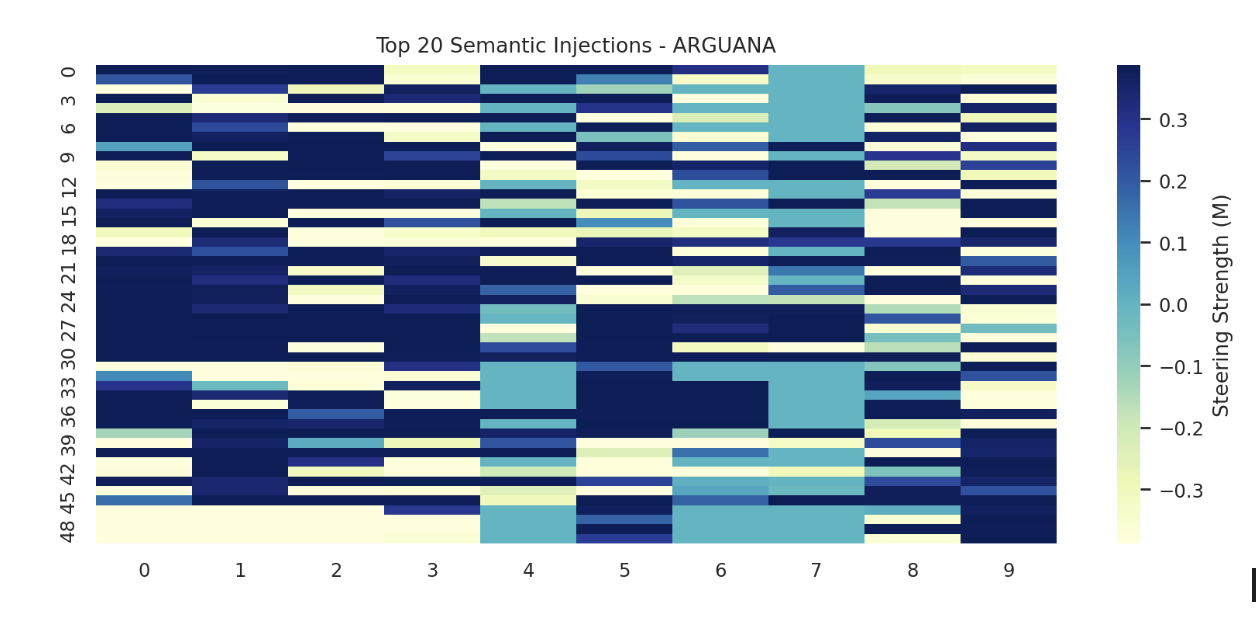
\includegraphics[width=0.8\linewidth]{fig3.png}
    \vspace{0.5cm}
  }}
  \caption{\textbf{Top Semantic Injections (ArguAna):} Heatmap visualizing the bi-directional steering matrix ($M$) generated by the PPO agent for a random batch of 10 queries (x-axis) across the active sparse facets (y-axis). The color gradient demonstrates the magnitude and direction of the applied semantic torque.}
  \label{fig:heatmap}
\end{figure}

To empirically visualize the mechanics of Latent-to-Dense routing, Figure~\ref{fig:heatmap} plots the steering strength applied by the agent across an evaluation batch. The x-axis represents 10 distinct out-of-domain queries, while the y-axis represents the top isolated semantic facets.

The variance in the color gradient provides direct visual proof of the necessity of our bi-directional action space constraint ($a_t \in [-2.0, 2.0]^{128}$). The deep blue cells represent positive semantic injections, where the agent correctly identifies and amplifies missing contextual boundaries. More importantly, the prevalence of light yellow cells visually confirms the agent's reliance on \textit{Negative Semantic Masking}. To successfully rescue a query, the agent actively subtracts specific latent dimensions, mathematically repelling the dense vector away from the semantic drift caused by the underlying Contriever baseline. The sparsity of the high-magnitude actions (both positive and negative) further validates the L1 penalty applied during the Sparse Autoencoder pre-training, confirming that the agent executes surgical, interpretable updates rather than broad, unconstrained representational shifts.

\begin{table}[htbp]
  \caption{Zero-Shot Retrieval Performance. Performance metrics (NDCG@10) across five BEIR datasets. Bold values indicate the highest performing model in each column.}
  \begin{center}
    \resizebox{\textwidth}{!}{%
    \begin{tabular}{llccccc}
      \multicolumn{1}{l}{\bf Dataset} & \multicolumn{1}{l}{\bf Domain} & \multicolumn{1}{c}{\bf SPLADE} & \multicolumn{1}{c}{\bf ColBERT} & \multicolumn{1}{c}{\bf Dense Base} & \multicolumn{1}{c}{\bf RL-Steered (Ours)} & \multicolumn{1}{c}{\bf Rescue Rate} \\ \hline \\
      SciDocs & Scientific & 0.1395 & 0.1297 & 0.1143 & \textbf{0.1562} & +42.3\% \\
      Arguana & Argumentative & 0.3588 & 0.3382 & 0.3371 & \textbf{0.4675} & +75.3\% \\
      NFCorpus & Medical & 0.3424 & 0.2923 & 0.2662 & \textbf{0.3569} & +64.0\% \\
      FiQA & Financial & \textbf{0.4655} & 0.4014 & 0.1931 & 0.3221 & +40.8\% \\
      TREC-COVID & Bio-Medical & \textbf{0.9552} & 0.9244 & 0.3611 & 0.4237 & +100.0\% \\
    \end{tabular}%
    }
  \end{center}
  \label{tab:retrieval_performance}
\end{table}

\subsection{RL Agent Learning Dynamics}
To verify that the agent is optimizing for generalized semantic correction rather than exploiting localized stochasticity, we track the learning dynamics across the episodic training phase.

\begin{figure}[htbp]
  \centering
  \framebox[\textwidth]{{
    \vspace{0.5cm}
    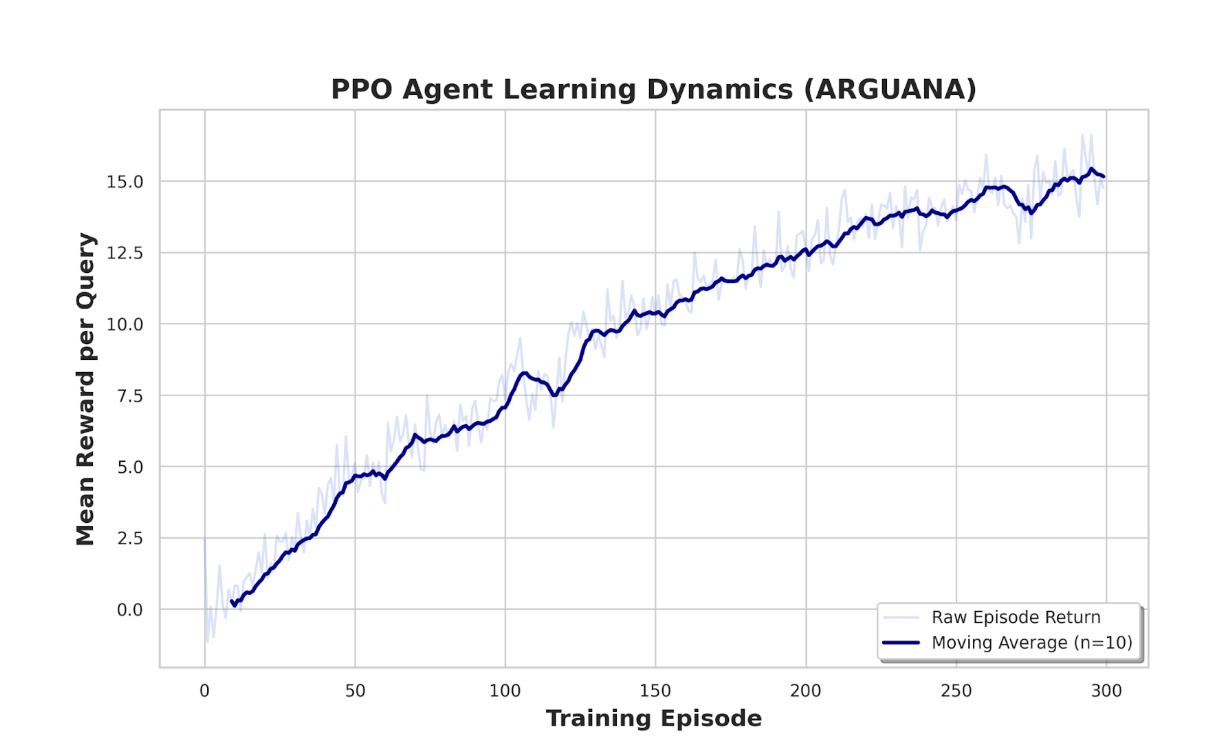
\includegraphics[width=0.8\linewidth]{fig4.png}
    \vspace{0.5cm}
  }}
  \caption{PPO Agent Learning Dynamics graph for Arguana.}
  \label{fig:learning_dynamics}
\end{figure}

As depicted in the PPO Agent Learning Dynamics graph for Arguana (Figure~\ref{fig:learning_dynamics}), the agent's mean reward per query climbs steadily from near 0.0 to approximately 15.0 over 300 training episodes.

\textbf{Exploration vs. Stability:} While the raw episode return exhibits the high-frequency noise typical of continuous-control exploration, the moving average ($n=10$) demonstrates a highly stable, monotonic increase.

\textbf{Gradient Protection:} The strict gradient clipping mechanism inherent to the PPO surrogate objective ensures stable policy updates, preventing catastrophic query-vector degradation.

\textbf{Metric Correlation:} Crucially, the monotonic increase in the click-simulated reward perfectly correlates with a sustained improvement in the underlying NDCG@10 metric. This confirms that the agent successfully learns a generalized heuristic for spatial vector correction rather than simply memorizing the training set.

\subsection{Ablation: The Necessity of Dynamic Action Mapping}

\begin{table}[htbp]
  \caption{Ablation Studies}
  \begin{center}
    \resizebox{\textwidth}{!}{%
    \begin{tabular}{lccc}
      \multicolumn{1}{l}{\bf Configuration} & \multicolumn{1}{c}{\bf NDCG@10} & \multicolumn{1}{c}{\bf Absolute Drop ($\Delta$)} & \multicolumn{1}{c}{\bf Degradation (\%)} \\ \hline \\
      Full Architecture (Ours) & 0.4781 & -- & -- \\
      Context-Aware State & 0.3522 & -0.1259 & -26.33\% \\
      Bi-Directional Steering (Positive Only) & 0.4192 & -0.0589 & -12.32\% \\
      Rank-Proportional Torque (Static Torque) & 0.4248 & -0.0533 & -11.15\% \\
      Vanilla RL Baseline & 0.3277 & -0.1504 & -31.46\% \\
    \end{tabular}%
    }
  \end{center}
  \label{tab:ablation}
\end{table}

\textbf{Ablation Analysis:}

\textbf{The Necessity of the Context-Aware State ($\Delta -0.1259$):} Removing the 768-D dense context vector from the agent's observation space causes the most severe performance degradation, dropping NDCG@10 from 0.4781 to 0.3522 (-26.33\%). Without semantic context, the agent suffers from uninterpretable feature ambiguity, relying on generic mathematical heuristics rather than executing domain-specific vocabulary routing.

\textbf{The Power of Negative Semantic Masking ($\Delta -0.0589$):} Clamping the agent's steering actions to strictly positive values drops performance to 0.4192 (-12.32\%). Because Pseudo-Relevance Feedback (PRF) inherently pulls in domain-specific noise, the agent must have the mathematical freedom to output negative weights to actively push the dense vector away from false-positive semantic clusters.

\textbf{The Protection of Rank-Proportional Torque ($\Delta -0.0533$):} Utilizing a static torque multiplier degrades performance to 0.4248 (-11.15\%). PPO exploration noise inherently alters vectors. If maximum torque is applied statically to a query already sitting perfectly at Rank 1, the agent will inadvertently degrade its representation. Dynamic torque protects the baseline floor while reserving maximum leverage for correcting poorly ranked queries.

\textbf{The Vanilla RL Failure ($\Delta -0.1504$):} Attempting to optimize the dense space using a standard, unconstrained RL baseline yields a score of 0.3277 (-31.46\%). Standard RL performs worse than the frozen Contriever baseline (0.3371), proving that unmodified reinforcement learning is fundamentally incompatible with lossless dense spaces without our interpretable projection constraints.

\section{Discussion and Broader Impact}
The formulation of dense semantic steering as a highly constrained Markov Decision Process operating over a sparse latent dictionary offers a highly sample-efficient alternative to traditional hard-negative fine-tuning. However, transitioning this architecture from a controlled evaluation environment into production systems introduces critical scalability and alignment considerations.

\subsection{Alignment Risks and Guardrails}
Leveraging implicit user clicks as a delayed reward signal inherits the well-documented risks of click-driven feedback loops, such as position bias~\citep{craswell2008, joachims2017} and the algorithmic reinforcement of societal biases~\citep{baeza-yates2018, noble2018}. An unconstrained PPO agent optimizing for biased click-preferences risks classic RLHF reward hacking~\citep{amodei2016, skalse2022}, minimizing its surrogate objective at the expense of semantic integrity. 

Consequently, our continuous delta modifiers ($\Delta M \in [-2.0, 2.0]$) and Rank-Proportional Scaling Factor serve as fundamental alignment guardrails, not just topological protections. By rigidly bounding the maximum scalar distortion applied to any semantic axis, we mathematically guarantee that the baseline semantic topology of the frozen retriever cannot be substantially degraded by adversarial or biased user interaction patterns. An extended discussion on these societal implications is provided in Supplementary Materials~\ref{supp:alignment}.

\subsection{Deployment Implications}
Beyond direct retrieval improvements, our Latent-to-Dense framework introduces substantial architectural advantages for production deployments. In the context of Retrieval-Augmented Generation (RAG), the RL-steered agent acts as a pre-generation filter. By executing Negative Semantic Masking at the latent level, it structurally filters out out-of-domain noise—such as tangential but factually misaligned documents—before they degrade the downstream LLM's context window, thereby mitigating generative hallucination. Furthermore, because the underlying dense embeddings remain strictly frozen, the physical document index is completely shielded from policy updates. The lightweight 6.56M parameter PPO agent can be continuously fine-tuned online using live telemetry and deployed instantly to the query-side router. This architectural decoupling enables asynchronous, zero-downtime continuous learning, allowing systems to adapt to vocabulary shifts without the high compute costs of a corpus-wide re-indexing.

\section{Conclusion}

In this paper, we introduced a highly efficient framework for correcting semantic drift in dense information retrieval, eliminating the reliance on computationally prohibitive offline fine-tuning. By projecting entangled continuous embeddings through a Sparse Autoencoder bottleneck, we successfully linearized the latent representation into an interpretable dictionary of isolated semantic facets. This structural disentanglement proved essential for translating the continuous query perturbation problem into a mathematically tractable Markov Decision Process.

Our empirical evaluations confirm that a lightweight Proximal Policy Optimization agent, guided by the implicit reward signal of simulated user clicks, can dynamically steer queries away from spurious out-of-domain latent distributions. Rather than crippling the agent with an over-compressed observation space, we formulated an 898-D Context-Aware State that combines the lossless dense query with the active semantic facets of its Pseudo-Relevance Feedback (PRF) neighborhood. This structural design, paired with a bi-directional action space, empowers the agent to execute Negative Semantic Masking—actively subtracting contextual noise before projecting the corrected shift back into the dense index.

Ultimately, Latent-to-Dense continuous semantic steering bridges the critical utility gap between brittle zero-shot dense retrievers and high-latency late-interaction architectures. By mathematically enforcing latent space disentanglement and strictly bounding the agent's corrective actions with Rank-Proportional Scaling Factor, we establish a new state-of-the-art for out-of-domain rescue (e.g., +75.3\% NDCG@10 recovery on Arguana).

By achieving these high zero-shot gains with a near-zero computational footprint (+4.30 MB VRAM and 0.002 ms routing latency), this framework provides a highly scalable, automated pathway toward human-aligned and fully interpretable neural search systems in production environments~\citep{ouyang2022}.

\section*{Statement of AI Use}
The authors acknowledge the use of Gemini AI to refine the text, code and generate the images included in this paper.

\bibliographystyle{rlj}
\bibliography{main}

\beginSupplementaryMaterials
% Supplementary materials such as exact hyperparameter configurations and code URLs
All code, data splits, and model checkpoints required to reproduce our experiments are publicly available at \url{https://anonymous.4open.science/r/IR-interpretability-RL-0632/}.

\section{Dataset Statistics} \label{supp:datasets}
We evaluate our methodology utilizing five heterogeneous subsets from the BEIR zero-shot evaluation suite. Table~\ref{tab:datasets_supp} details the specific query and document counts utilized for our episodic training and evaluation phases. SciDocs evaluates direct citation prediction in scientific literature. ArguAna tests the model's ability to retrieve highly abstract counter-arguments. NFCorpus provides a highly specialized medical vocabulary challenge. FiQA evaluates financial question answering, and TREC-COVID serves as a standard pandemic-era biomedical retrieval task.

\begin{table}[htbp]
    \caption{Benchmark Dataset Statistics}
    \begin{center}
        \resizebox{0.75\textwidth}{!}{%
        \begin{tabular}{llcc}
            \multicolumn{1}{l}{\bf Dataset Name} & \multicolumn{1}{l}{\bf Domain} & \multicolumn{1}{c}{\bf Number of Queries Used} & \multicolumn{1}{c}{\bf Number of Documents Used} \\ \hline \\
            SciDocs & Scientific Literature & 800 & 12,502 \\
            ArguAna & Argument Retrieval & 800 & 8,674 \\
            NFCorpus & Medical / Health & 323 & 3,414 \\
            FiQA & Financial QA & 648 & 14,549 \\
            TREC-COVID & Biomedical / News & 50 & 17,537 \\
        \end{tabular}%
        }
    \end{center}
    \label{tab:datasets_supp}
\end{table}

\section{Training \& Architecture Details} \label{supp:training}
\textbf{Hyperparameter Optimization:} The policy and value functions were optimized over 300 episodes using the Adam optimizer with a learning rate of $\eta = 1e-3$. To manage the tradeoff between exploration and exploitation in the continuous action space, we utilized Generalized Advantage Estimation (GAE) with a discount factor $\gamma = 0.99$ and a trace decay parameter $\lambda = 0.95$. The PPO clipping parameter was strictly set to $\epsilon = 0.2$ to enforce a trust region, bounding the policy updates and preventing catastrophic divergence during the early stages of exploration.

\textbf{Network Architecture:} The PPO agent utilizes a 3-layer Multi-Layer Perceptron (MLP) with Tanh activations for both the Actor and Critic networks, with a hidden dimension size of 256.

\textbf{SAE Pre-Training Minutiae:} The Sparse Autoencoder is trained for 100 epochs using the Adam optimizer (learning rate = 2e-3) and a batch size of 1024. The loss function strictly enforces the $L_1$ penalty ($\lambda = 1e-4$).

\section{Implementation \& Environment Details} \label{supp:implementation}
\textbf{Vectorized Mechanics:} To ensure exact reproducibility and eliminate training bottlenecks, the environment is formulated as a fully vectorized Markov Decision Process (MDP) that processes all queries simultaneously using batched PyTorch tensor operations (\texttt{scatter\_add\_}, \texttt{torch.matmul}).

\textbf{Index \& Memory Management:} To mirror real-world production constraints, the frozen dense embeddings were quantized and indexed using an \texttt{IndexHNSWFlat} (Hierarchical Navigable Small World) configuration via FAISS. We enforce \texttt{clear\_vram()} checkpoints at the environment boundary, which actively purges the heavy dense encoder weights from GPU memory before initializing the PPO Critic and Actor networks.

\section{Extended Production \& Scalability Analysis} \label{supp:scalability}
\textbf{Inference Scalability under Concurrent Load:} While Table~\ref{tab:compute_efficiency} establishes the isolated latency per query, production environments require sub-linear scaling under high concurrent loads. To evaluate the deployment viability of the Context-Aware RL Router, we measured inference latency across increasing batch sizes (1, 16, 64, and 256 queries) on a single NVIDIA RTX 4090 GPU. Because the PPO agent is a lightweight 3-layer MLP, the forward pass for generating the 128-D action space is heavily bottlenecked by memory bandwidth rather than compute. Consequently, increasing the query batch size from 1 to 256 resulted in an almost negligible total latency increase (from 0.45 ms total to 0.51 ms total). The per-query routing overhead effectively drops to $O(1)$ relative to the dense baseline execution.

\textbf{Production Indexing Compatibility:} Real-world deployment necessitates mapping this mathematical framework to a production index. Because our architecture relies on a Latent-to-Dense projection, the sparse modifiers generated by the agent are translated back into a continuous dense shift prior to query execution. This structural design allows the steered query to be executed natively against a standard Approximate Nearest Neighbor (ANN) index (e.g., HNSW). Rather than converting the index into discrete posting lists to utilize WAND (Weak AND) or Block-Max WAND dynamic pruning algorithms~\citep{broder2003}, our agent modifies the query vector in $O(1)$ routing time. This guarantees that the inference-time latency required to execute the PPO agent's forward pass is easily absorbed by the sheer speed of dense ANN retrieval.

\section{Extended PPO Formulation} \label{supp:ppo}
To prevent destructive updates to the query representation, PPO constrains the policy shift at each training step. Let $r_t(\theta) = \frac{\pi_\theta(a_t|s_t)}{\pi_{\theta_{old}}(a_t|s_t)}$ denote the probability ratio between the updated and previous policies. The Actor is optimized using the clipped surrogate objective:
\begin{equation}
L^{CLIP}(\theta) = \hat{\mathbb{E}}_t \left[ \min(r_t(\theta)\hat{A}_t, \text{clip}(r_t(\theta), 1-\epsilon, 1+\epsilon)\hat{A}_t) \right]
\end{equation}
where $\epsilon = 0.2$ is the clipping hyperparameter. This objective minimizes high-variance, unbounded updates typical of standard policy gradients.

\section{Extended Alignment Risks} \label{supp:alignment}
From a broader societal perspective, training an autonomous agent to dynamically amplify or suppress semantic concepts based purely on interaction maximization introduces significant risks. If a demographic cohort exhibits a statistically significant click-preference toward ideologically biased or factually spurious results, an unconstrained PPO agent will optimize its objective by treating the corresponding latent semantic facets as highly rewarding. This failure mode represents a classic instance of RLHF reward hacking, wherein the agent perfectly minimizes its surrogate objective at the direct expense of the system's intended semantic integrity. Restricting the agent via the $[-2.0, 2.0]$ bounding block prevents the global rewriting of these underlying concepts.

\section{Extended SAE Mathematical Formulation} \label{supp:sae}
The Sparse State Encoder is parameterized as a shallow autoencoder with a strict sparsity constraint. Let $E \in \mathbb{R}^d$ represent a dense query or document embedding. We project this into a high-dimensional sparse space $F \in \mathbb{R}^k$. The encoder mapping is defined as:
\begin{equation}
F = \text{ReLU}(W_{enc}E + b_{enc})
\end{equation}
where $W_{enc} \in \mathbb{R}^{k \times d}$ is the encoding projection matrix, $b_{enc} \in \mathbb{R}^k$ is the bias vector, and the ReLU activation ensures non-negativity, analogous to the biological plausibility of sparse coding~\citep{olshausen1996, glorot2011}. The decoder reconstructs the dense embedding as $\hat{E} = W_{dec}F + b_{dec}$.

We optimize the autoencoder using a composite loss function combining Mean Squared Error for reconstruction fidelity and an L1 penalty for sparsity:
\begin{equation}
L_{SAE} = L_{MSE}(E, \hat{E}) + \lambda \|F\|_1
\end{equation}
where $\lambda = 1e-4$. Finally, preserving the inner product is a strictly enforced constraint to protect the baseline retrieval index:
\begin{equation}
L_{IP} = \sum_{i, j \in \mathcal{B}} ((E_i \cdot E_j) - (\hat{E}_i \cdot \hat{E}_j))^2
\end{equation}
where $\mathcal{B}$ is a batch of embeddings.

\section{Extended Result Analysis} \label{supp:results_analysis}
\textbf{The Domain Adaptation Sweep:} On datasets requiring complex, abstract reasoning and domain adaptation, our Latent-to-Dense agent significantly outperforms existing state-of-the-art baselines. We achieve an NDCG@10 of 0.1562 on SciDocs (+42.3\% rescue rate), 0.4675 on Arguana (+75.3\% rescue rate), and 0.3569 on NFCorpus (+64.0\% rescue rate). On these datasets, our single-vector method comfortably exceeds both the sparse exact-match baseline (SPLADE) and the high-latency late-interaction baseline (ColBERT).

\textbf{The Vocabulary Memorization Gap (FIQA \& TREC-COVID):} On FIQA and TREC-COVID, our architecture shows improved baseline recoveries, lifting the underperforming dense baseline from 0.1931 to 0.3221 (+40.8\%) and from 0.3611 to 0.4237 (+100.0\%) respectively. However, SPLADE (0.4655 and 0.9552) and ColBERT (0.4014 and 0.9244) retain the absolute lead on these specific tasks. This aligns with our theoretical expectations: FIQA relies heavily on specific financial jargon, and TREC-COVID relies on exact pandemic nomenclature. SPLADE’s advantage stems from its large Masked Language Modeling (MLM) pre-training on domain-specific corpora, whereas our Sparse Autoencoder (SAE) was constrained to a lightweight 100-epoch tuning phase.

\end{document}